\documentclass{beamer}
\usetheme{Madrid}

%------------------------------------------------------------------- PACKAGES -
\usepackage[brazil]{babel}     %permite acentuação automática para o Portugues do Brasil,
\usepackage[T1]{fontenc}       %permite a hifenização correta em Portugues
\usepackage[utf8]{inputenc} %permite a inserção de acentos (Windows)
\usepackage{colortbl}
%\usepackage{amsfonts}
%\usepackage{graphicx}
%\usepackage{rotating}

%\usepackage{float}
%\usepackage{fancyvrb}

%---------------------------------------------------------------- DEFINITIONS -
%
%\def\dis{\displaystyle}
%\def\ol{\overline}
%\newcommand{\ang}[1]{\left\langle #1 \right\rangle}
%\newcommand{\transp}[2]{\input{#1#2}}
%
%\FontTitle{\large}{BW}
%FontTitle{\large}
%\hypersetup{pdfpagemode=FullScreen}


%---------------------------------------------------------------------- COVER -
\title[]{Competições de Programação, por que você ainda não está participando?}
\author[{\tiny Paulo Cezar}]{Paulo Cezar Pereira Costa}
\institute[{\tiny INF/UFG}]{Instituto de Informática\\
           Universidade Federal de Goiás}
%\date[]{}

%\title{Maratona de Programação}
%%\subtitle{\normalsize Instituto de Informática -- UFG}
%\author{Humberto Longo}
%% \email{longo@inf.ufg.br}
%% \institution{Instituto de Informática \\ Universidade Federal de Goiás}%
%% \slideCaption{Maratona de Programação}


\AtBeginSection[]
{
\begin{frame}<beamer>
\frametitle{}
\begin{center}
	\begin{minipage}{.7\textwidth}
	\begin{block}{}
		\centering
		\huge
		\tt
		{\usebeamercolor[bg]{block title} \insertsection}
	\end{block}
	\end{minipage}
\end{center}
\end{frame}
}

\includeonly
{
competicoes,
maratona,
preparacao,
}


\begin{document}

\maketitle

\section{Introdução}
%- - - - - - - - - - - - - - - - - - - - - - - - - - - - - - - - - SLIDE -
\begin{frame}
\frametitle{Competições de Programação}
\begin{block}{O que são?}
\begin{itemize}
	\item São competições onde um programador, ou grupo de programadores, deve apresentar soluções computacionais corretas para um dado conjunto de problemas.
	\begin{itemize}
		\item A correção é automatizada e realizada por meio de testes:
		\begin{itemize}
			\item um conjunto de dados de entrada.
			\item um meio de validar a resposta gerada.
		\end{itemize}
		\item O programa solução deve:
		\begin{itemize}
			\item gerar um conjunto de dados de saída correspondente ao conjunto de dados recebido na entrada.
			\item respeitar limites de tempo de execução e de quantidade de memória usada.
			\item o resultado do programa deve ser validado corretamente nos testes realizados.
		\end{itemize}
	\end{itemize}
\end{itemize}
\end{block}
\end{frame}
%- - - - - - - - - - - - - - - - - - - - - - - - - - - - - - - - - SLIDE -
\begin{frame}
\frametitle{Competições de Programação}
\begin{block}{Por que é Bom?}
\begin{itemize}
	\item Essas competições estimulam a capacidade de resolver problemas computacionais rápida e eficientemente, uma das principais habilidades exigidas de um profissional de Computação.
	\item Você ganha motivação para estudar algoritmos e estruturas de dados.
    \item Estimulam o raciocínio lógico, o que acaba resultando em um melhor desempenho acadêmico.
	\item Você busca conhecer todos os recursos das linguagens de programação.
	\item Possibilidade de viagem para vários destinos do Brasil e do mundo.
    \item Boas colocações nessas competições enriquecem seu curriculo como programador e resolvedor de problemas, o que é muito valorizado por grandes empresas da área.
	\item É sempre bom competir!
\end{itemize}
\end{block}
\end{frame}

%- - - - - - - - - - - - - - - - - - - - - - - - - - - - - - - - -
%- - - - - - - - - - - - - - - - - - - - - - - - - - - - - - - - - SLIDES - SNCT
\begin{frame}
\frametitle{Competições de Programação}
\begin{block}{Por que é Bom?}
\begin{center}
	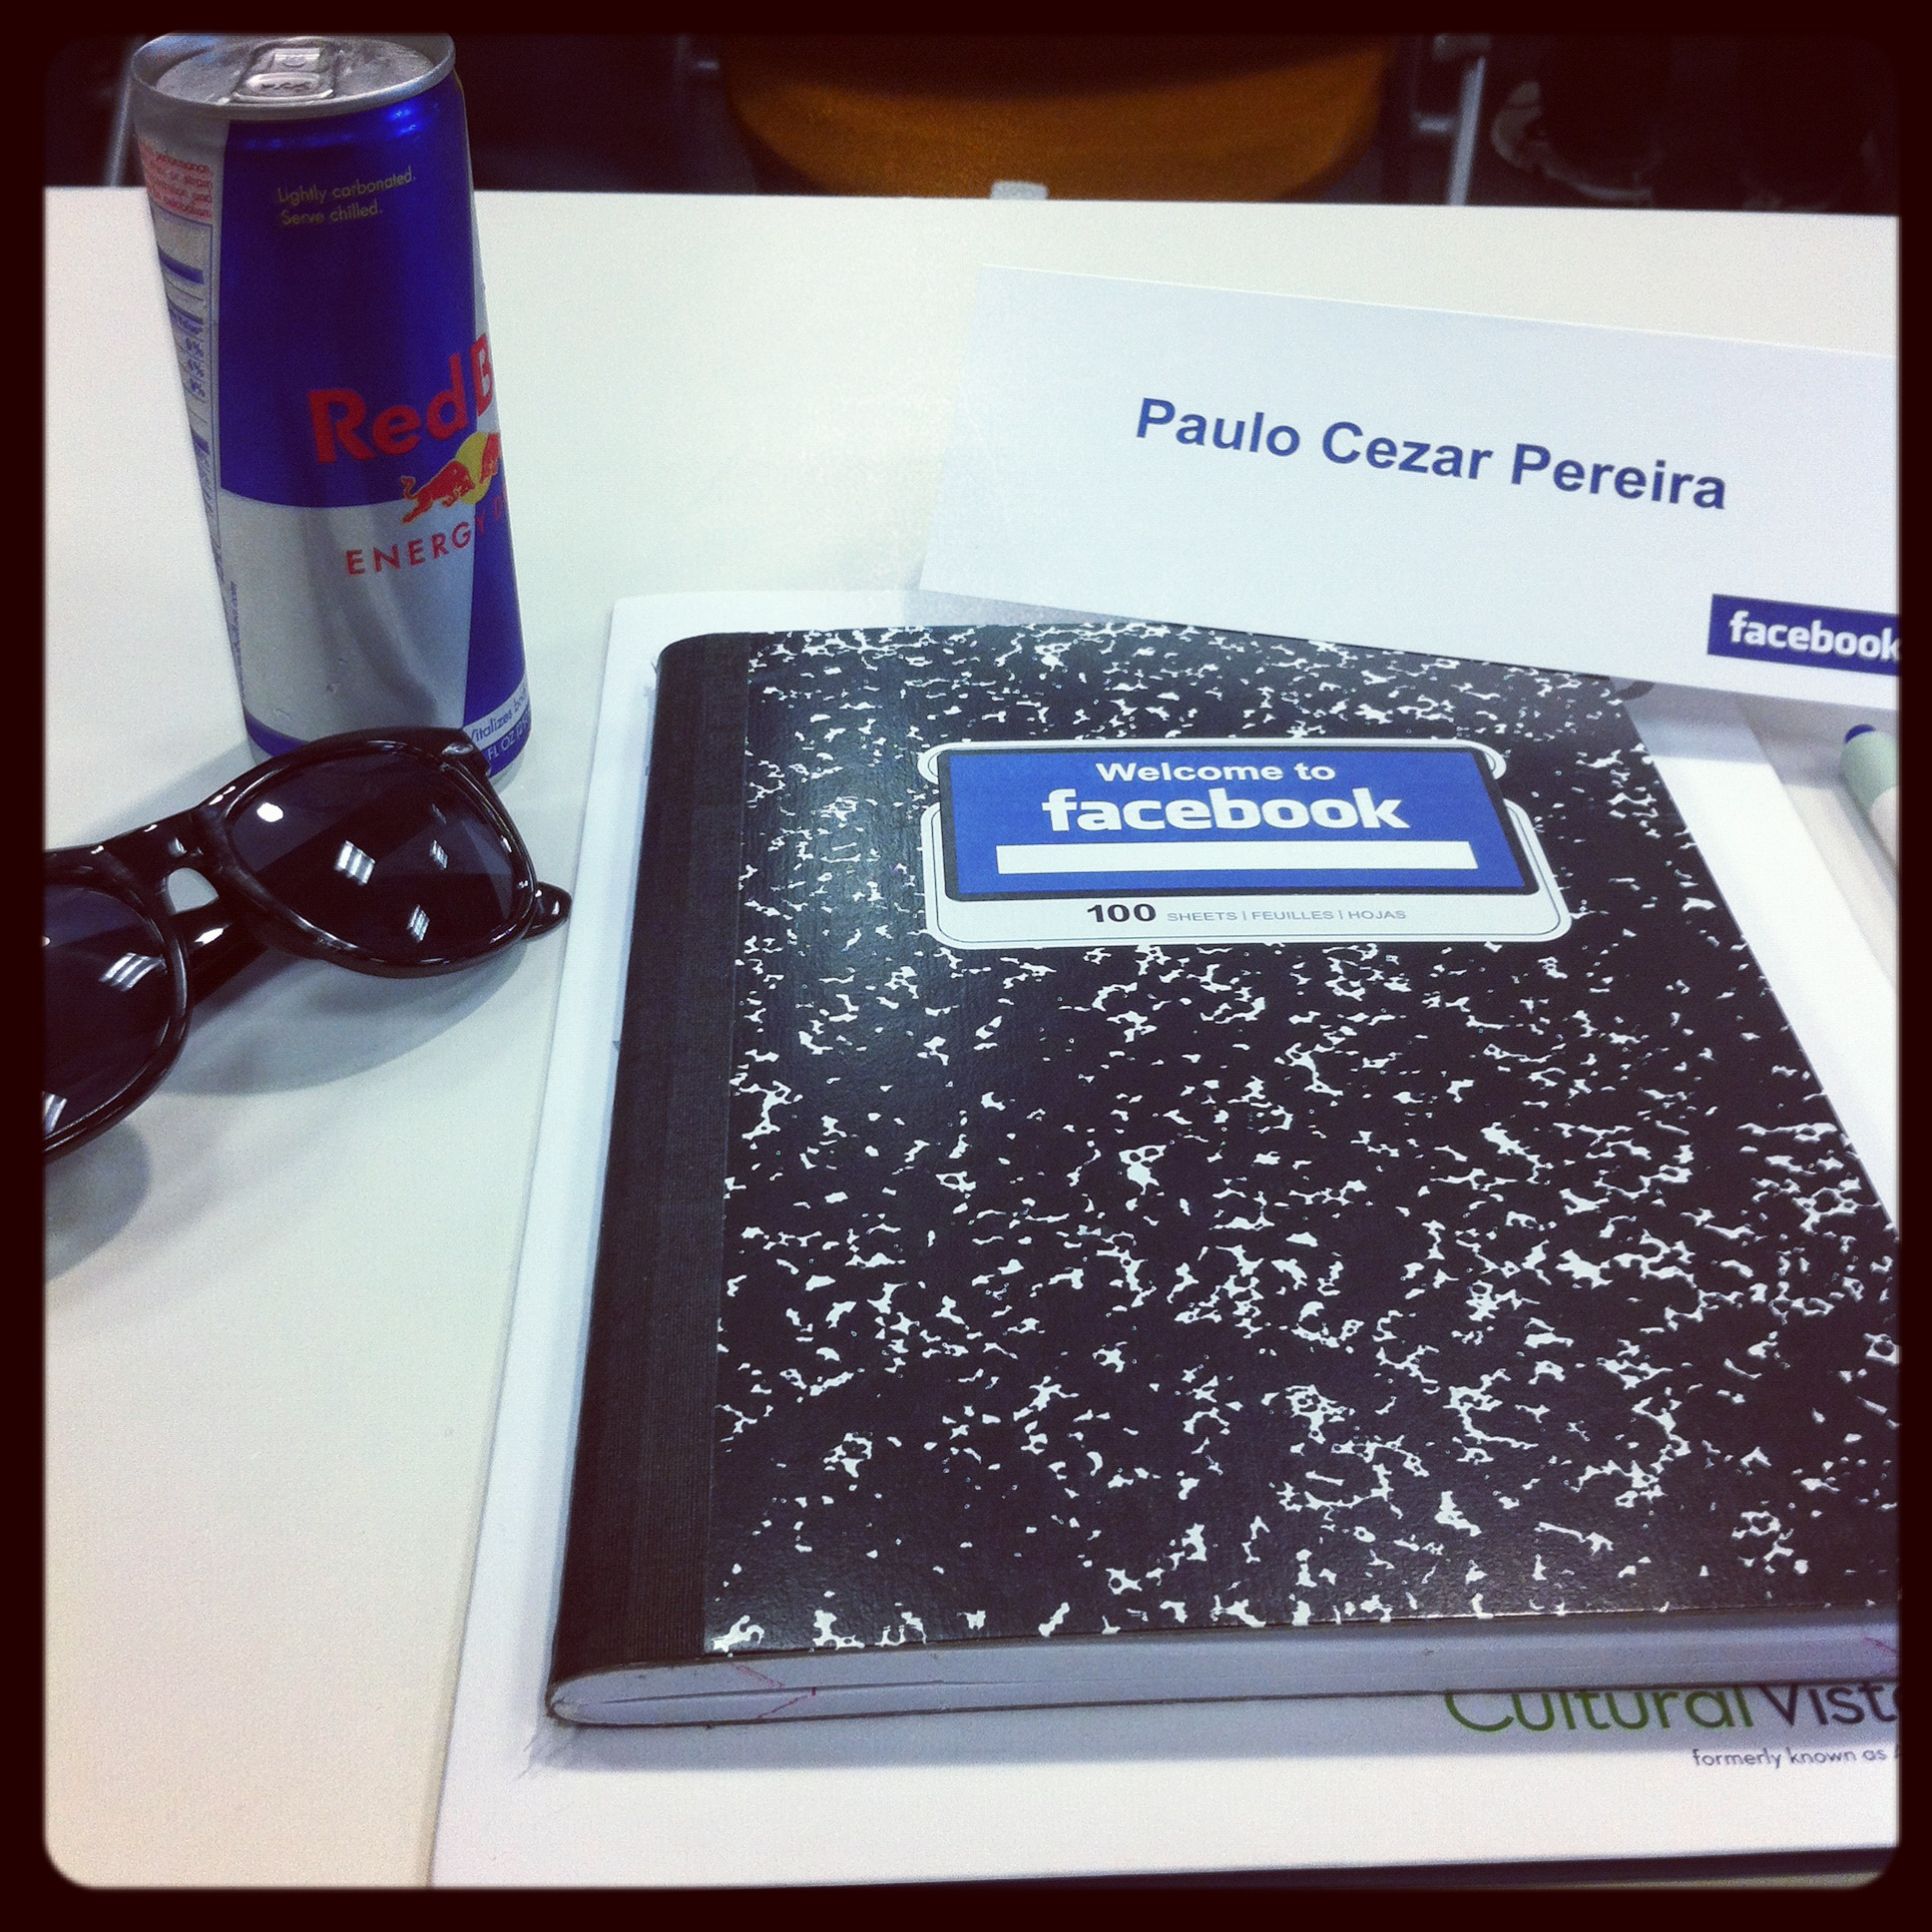
\includegraphics[height=.7\textheight]{sntc/IMG_1649.JPG}
\end{center}
\end{block}
\end{frame}
\begin{frame}
\frametitle{Competições de Programação}
\begin{block}{Por que é Bom?}
\begin{center}
	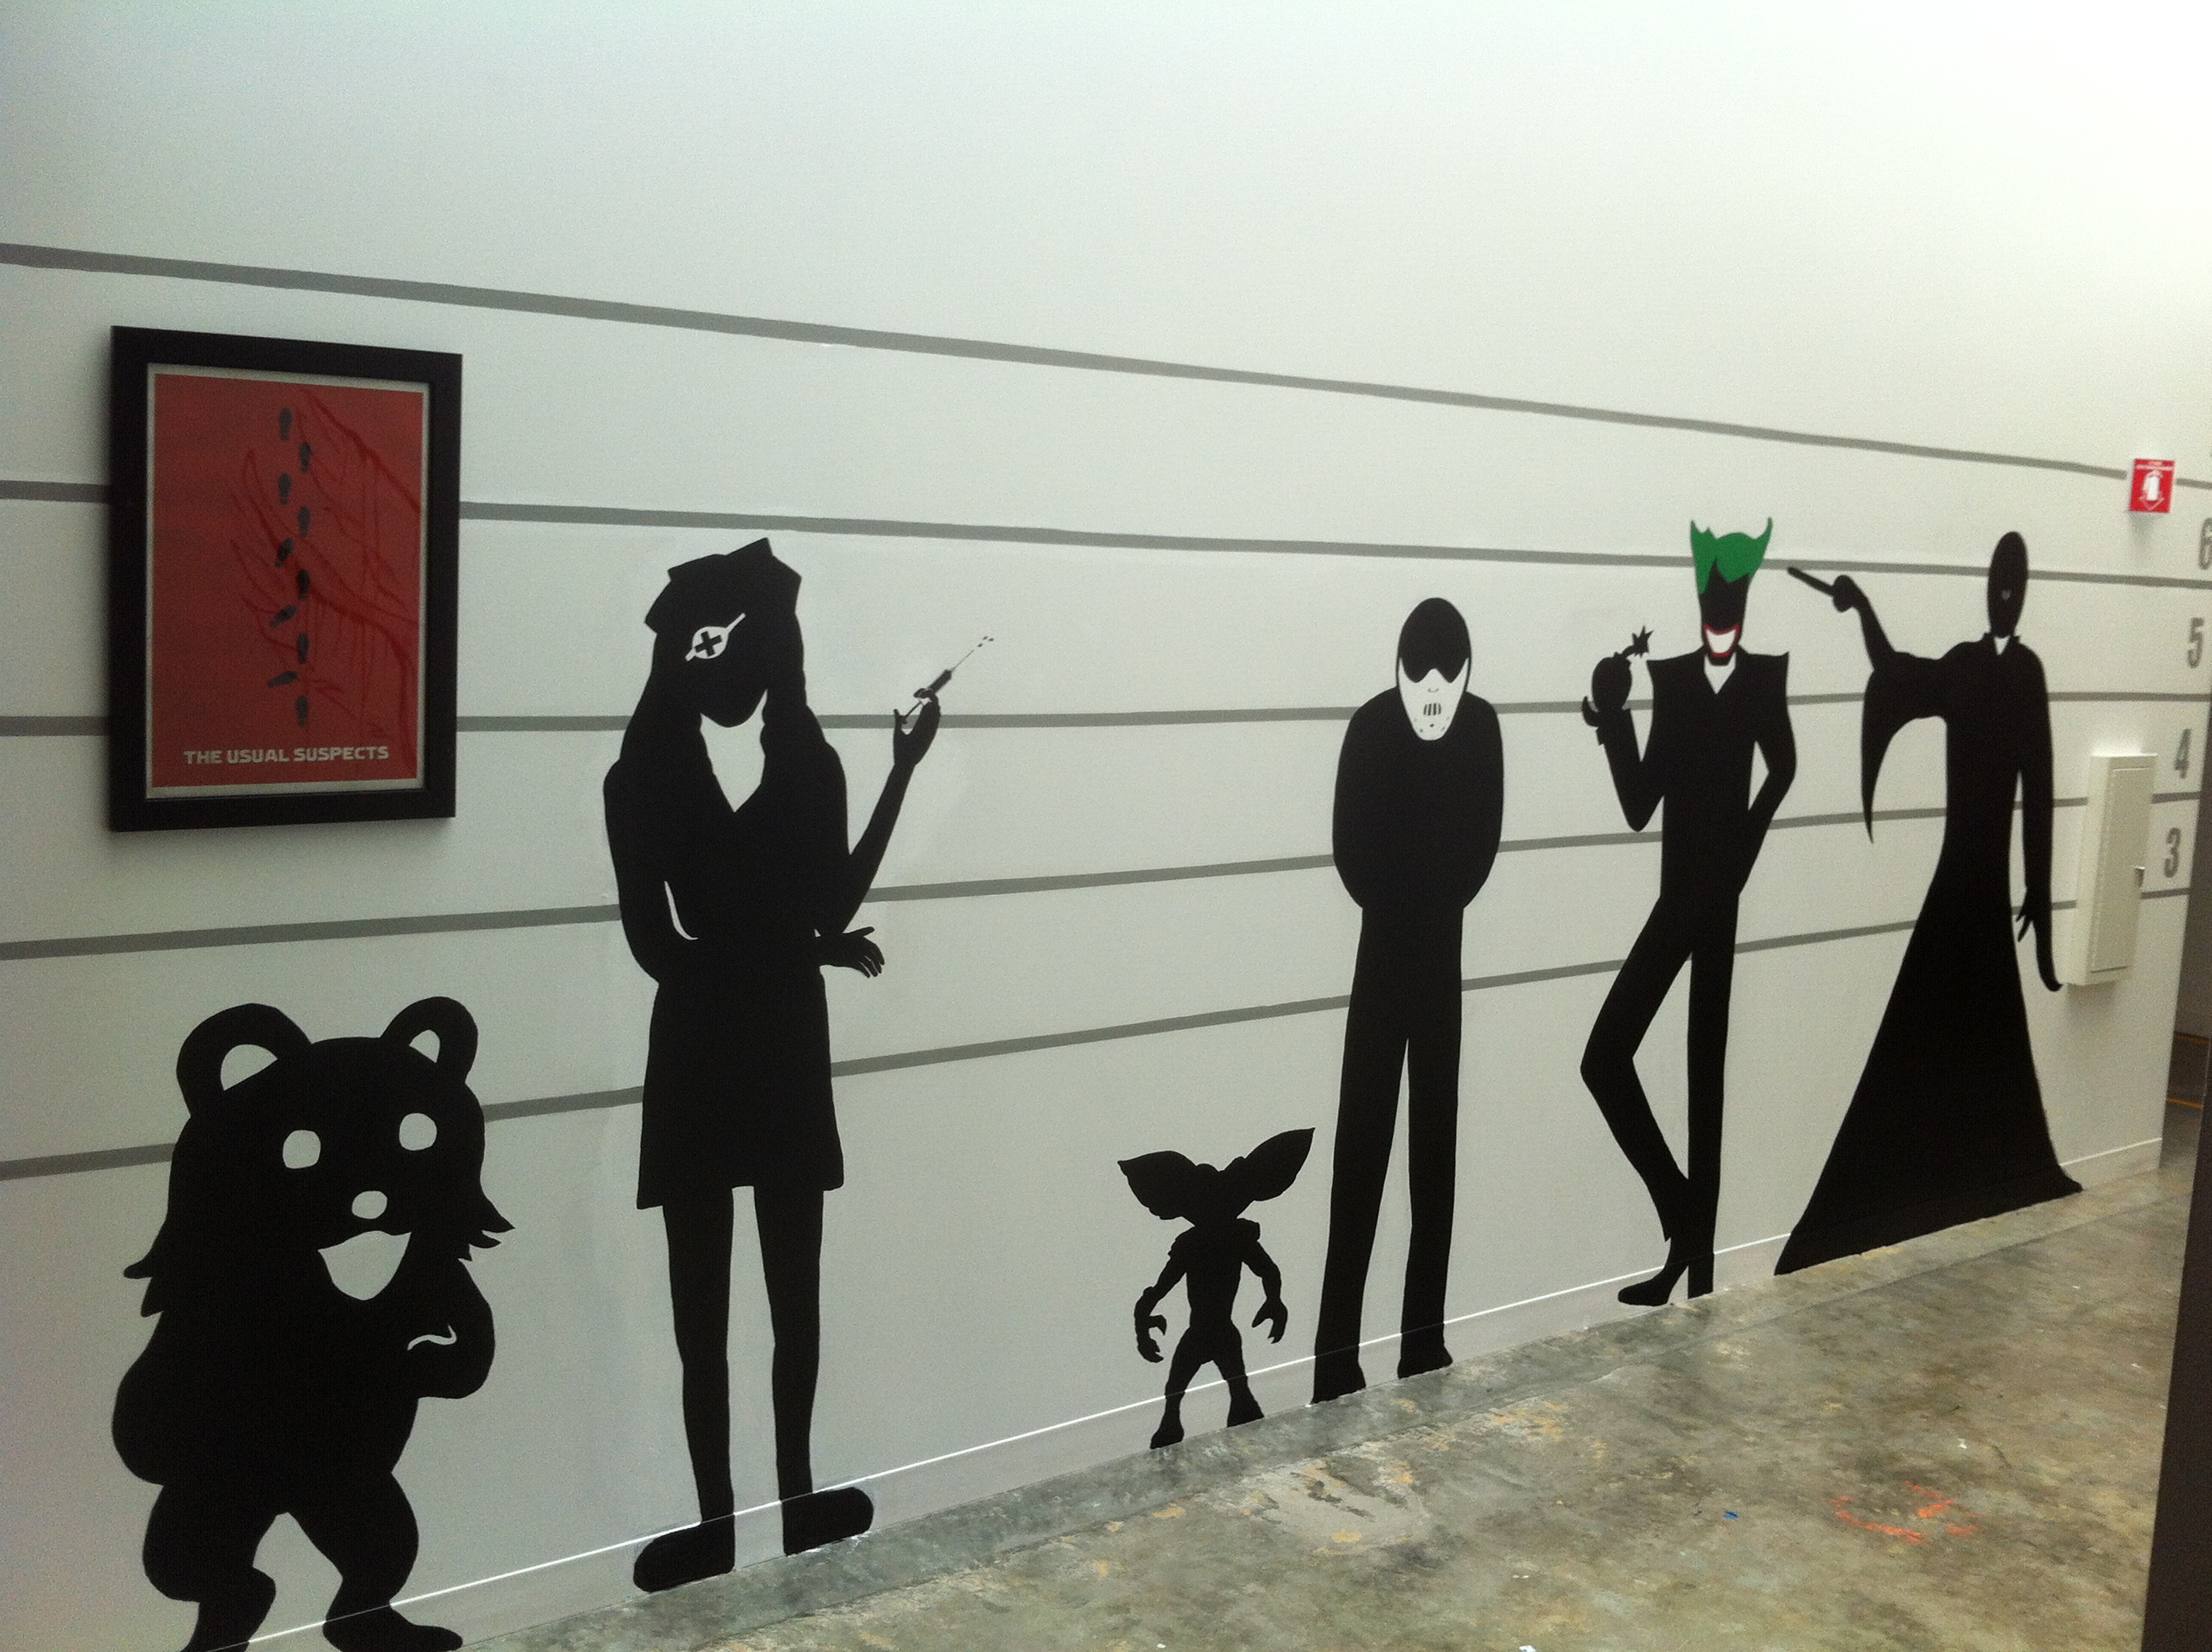
\includegraphics[width=.7\textwidth]{sntc/IMG_2040.JPG}
\end{center}
\end{block}
\end{frame}
\begin{frame}
\frametitle{Competições de Programação}
\begin{block}{Por que é Bom?}
\begin{center}
	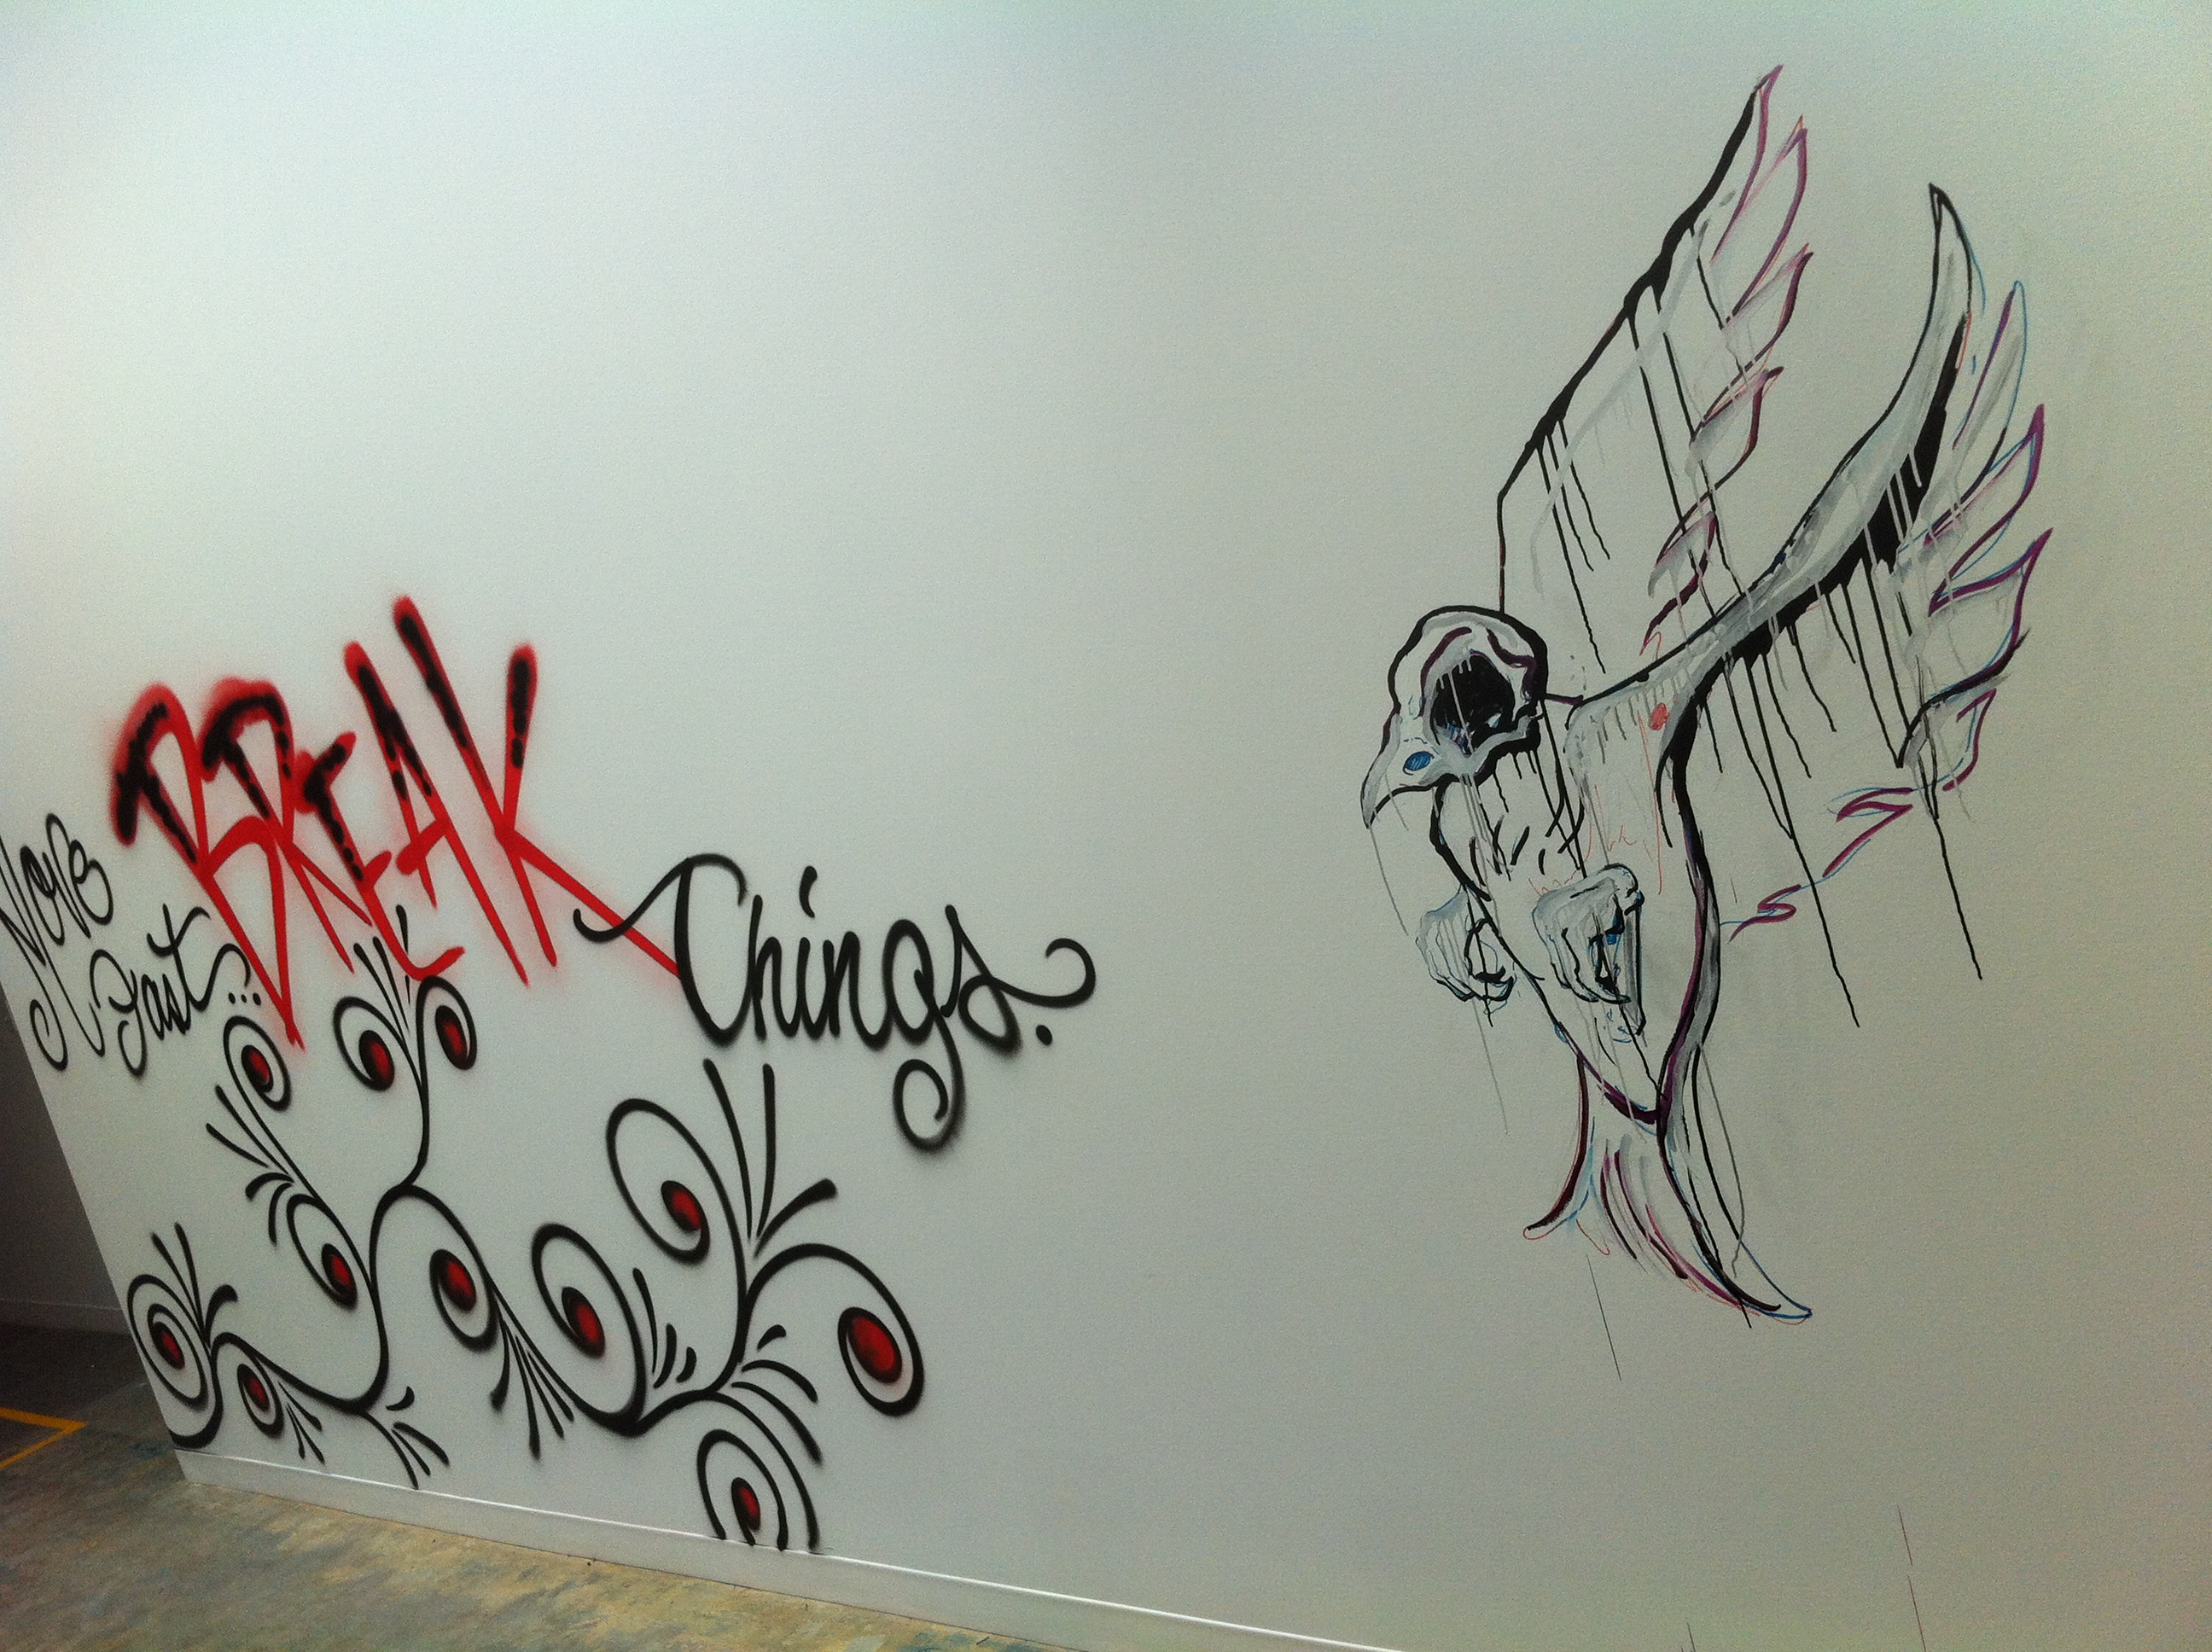
\includegraphics[width=.7\textwidth]{sntc/IMG_2045.JPG}
\end{center}
\end{block}
\end{frame}
\begin{frame}
\frametitle{Competições de Programação}
\begin{block}{\tiny{Por que é Bom?}}
\begin{center}
	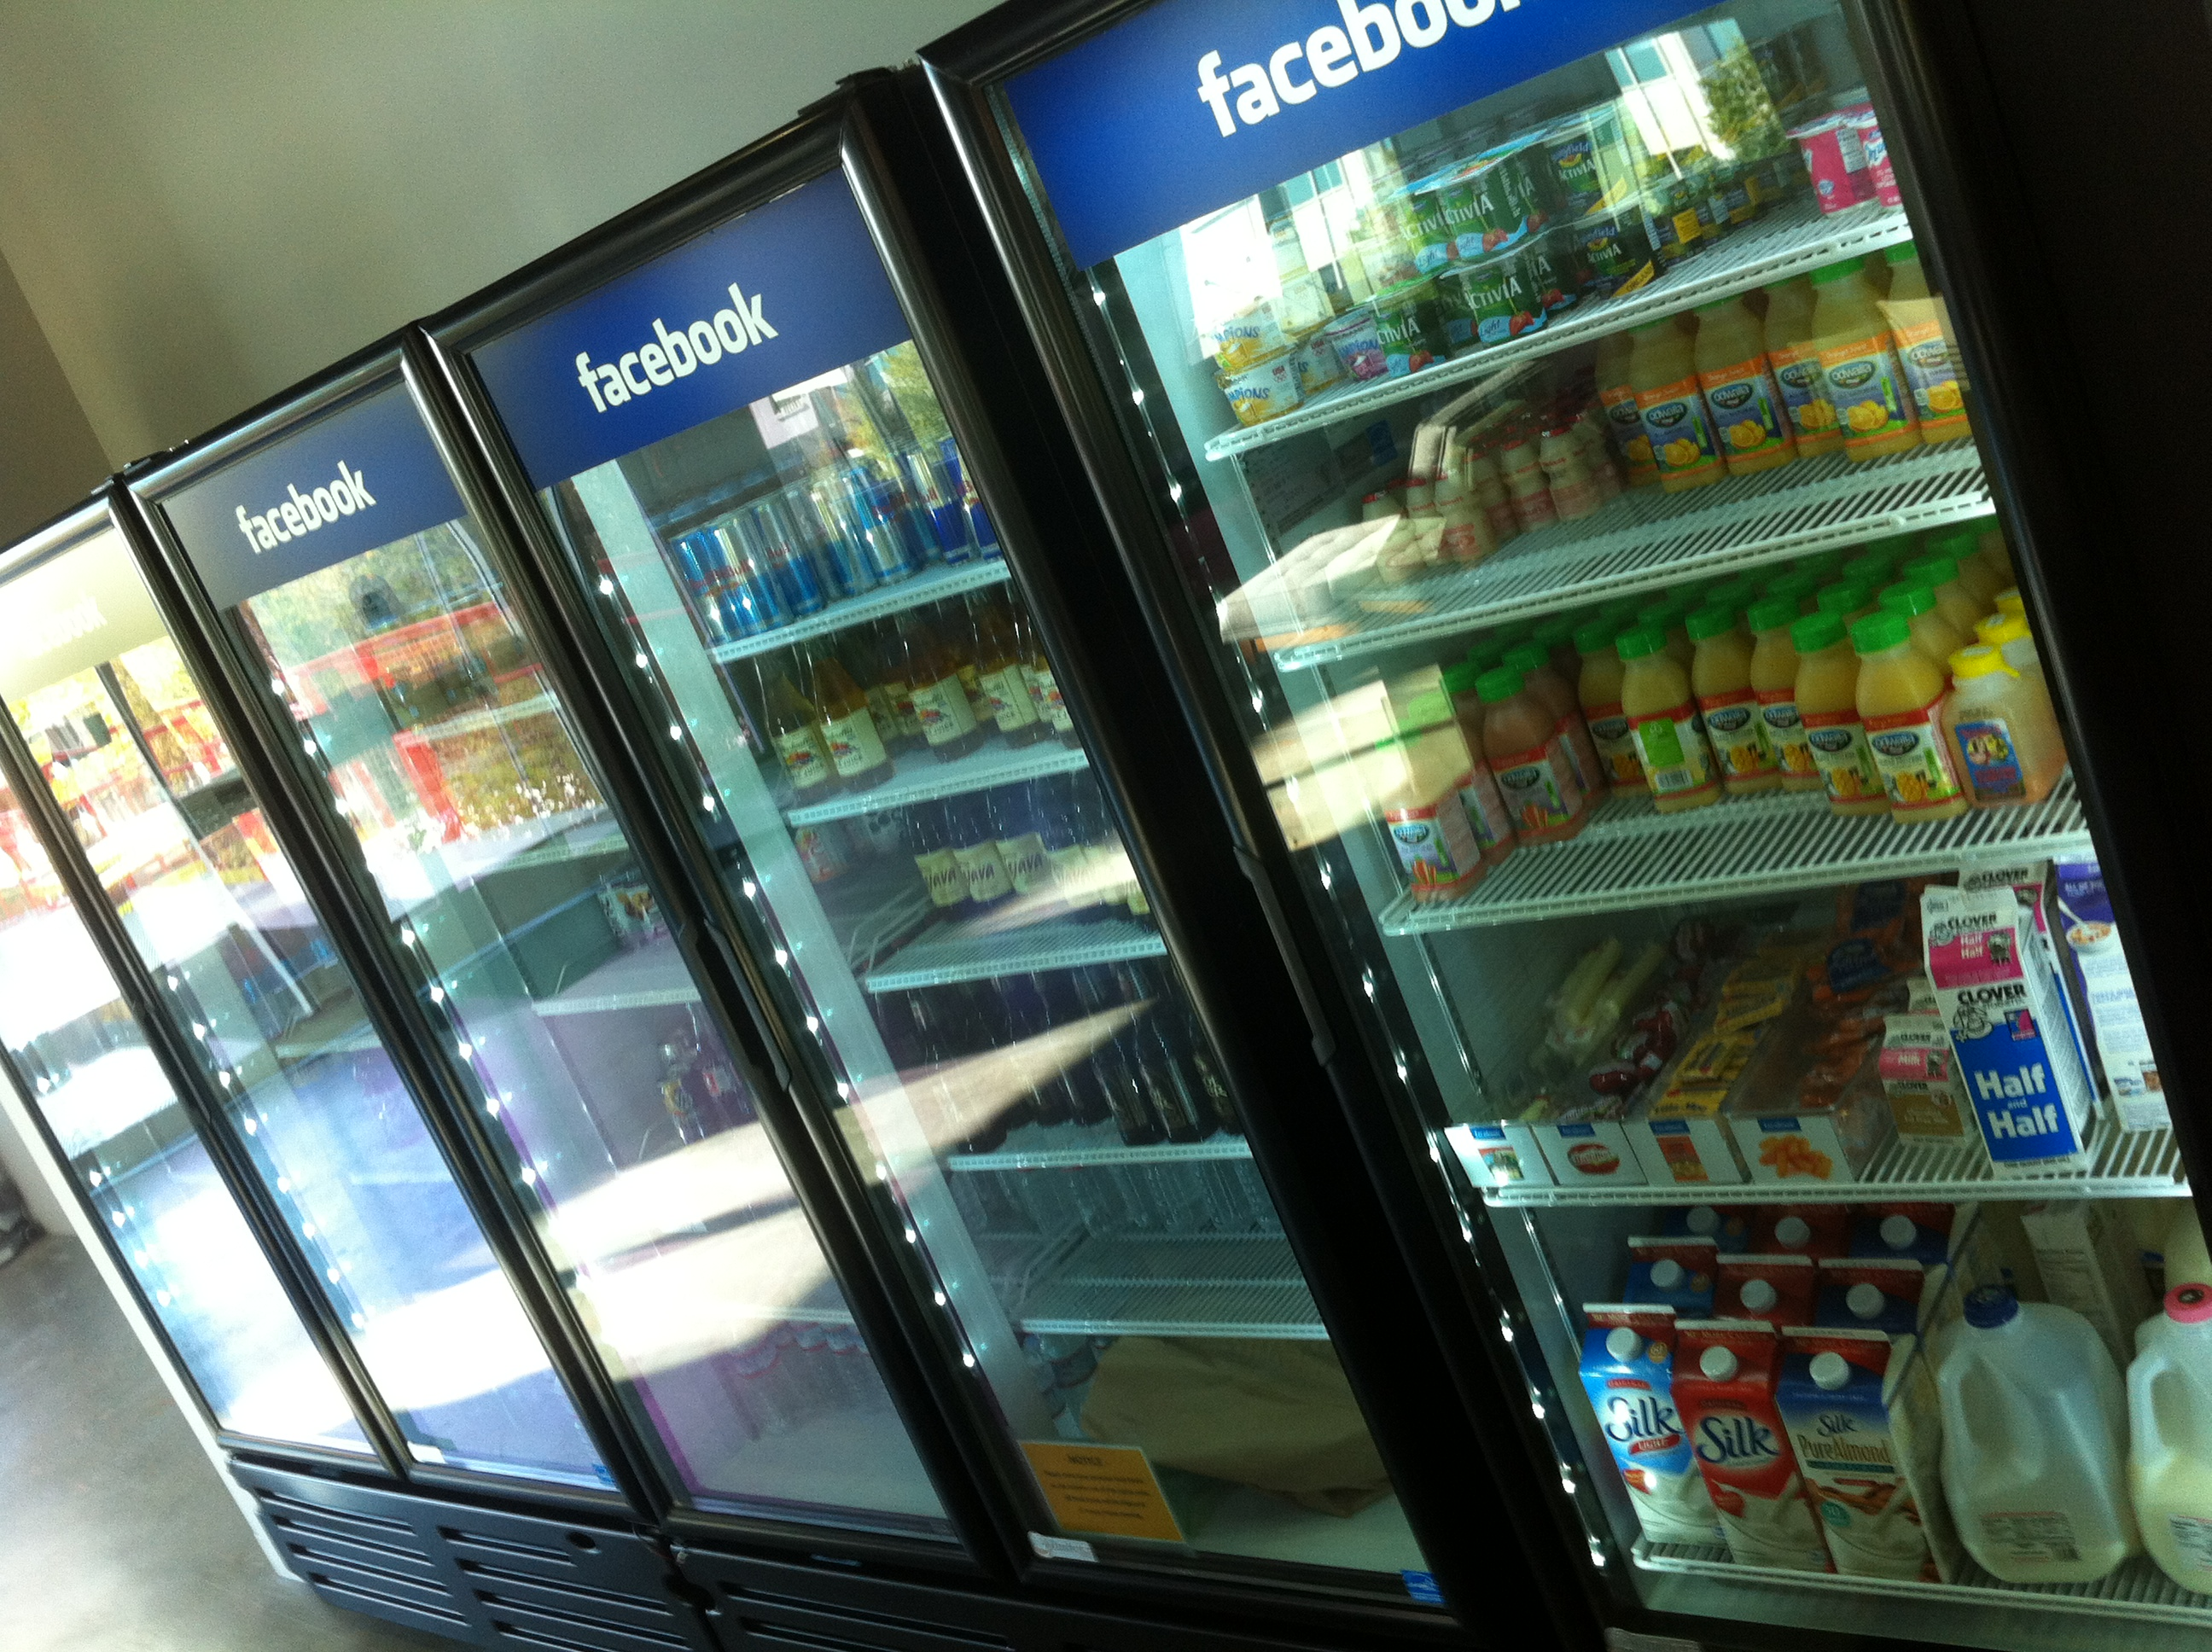
\includegraphics[width=.7\textwidth]{sntc/IMG_2049.JPG}
\end{center}
\end{block}
\end{frame}
\begin{frame}
\frametitle{Competições de Programação}
\begin{block}{Por que é Bom?}
\begin{center}
	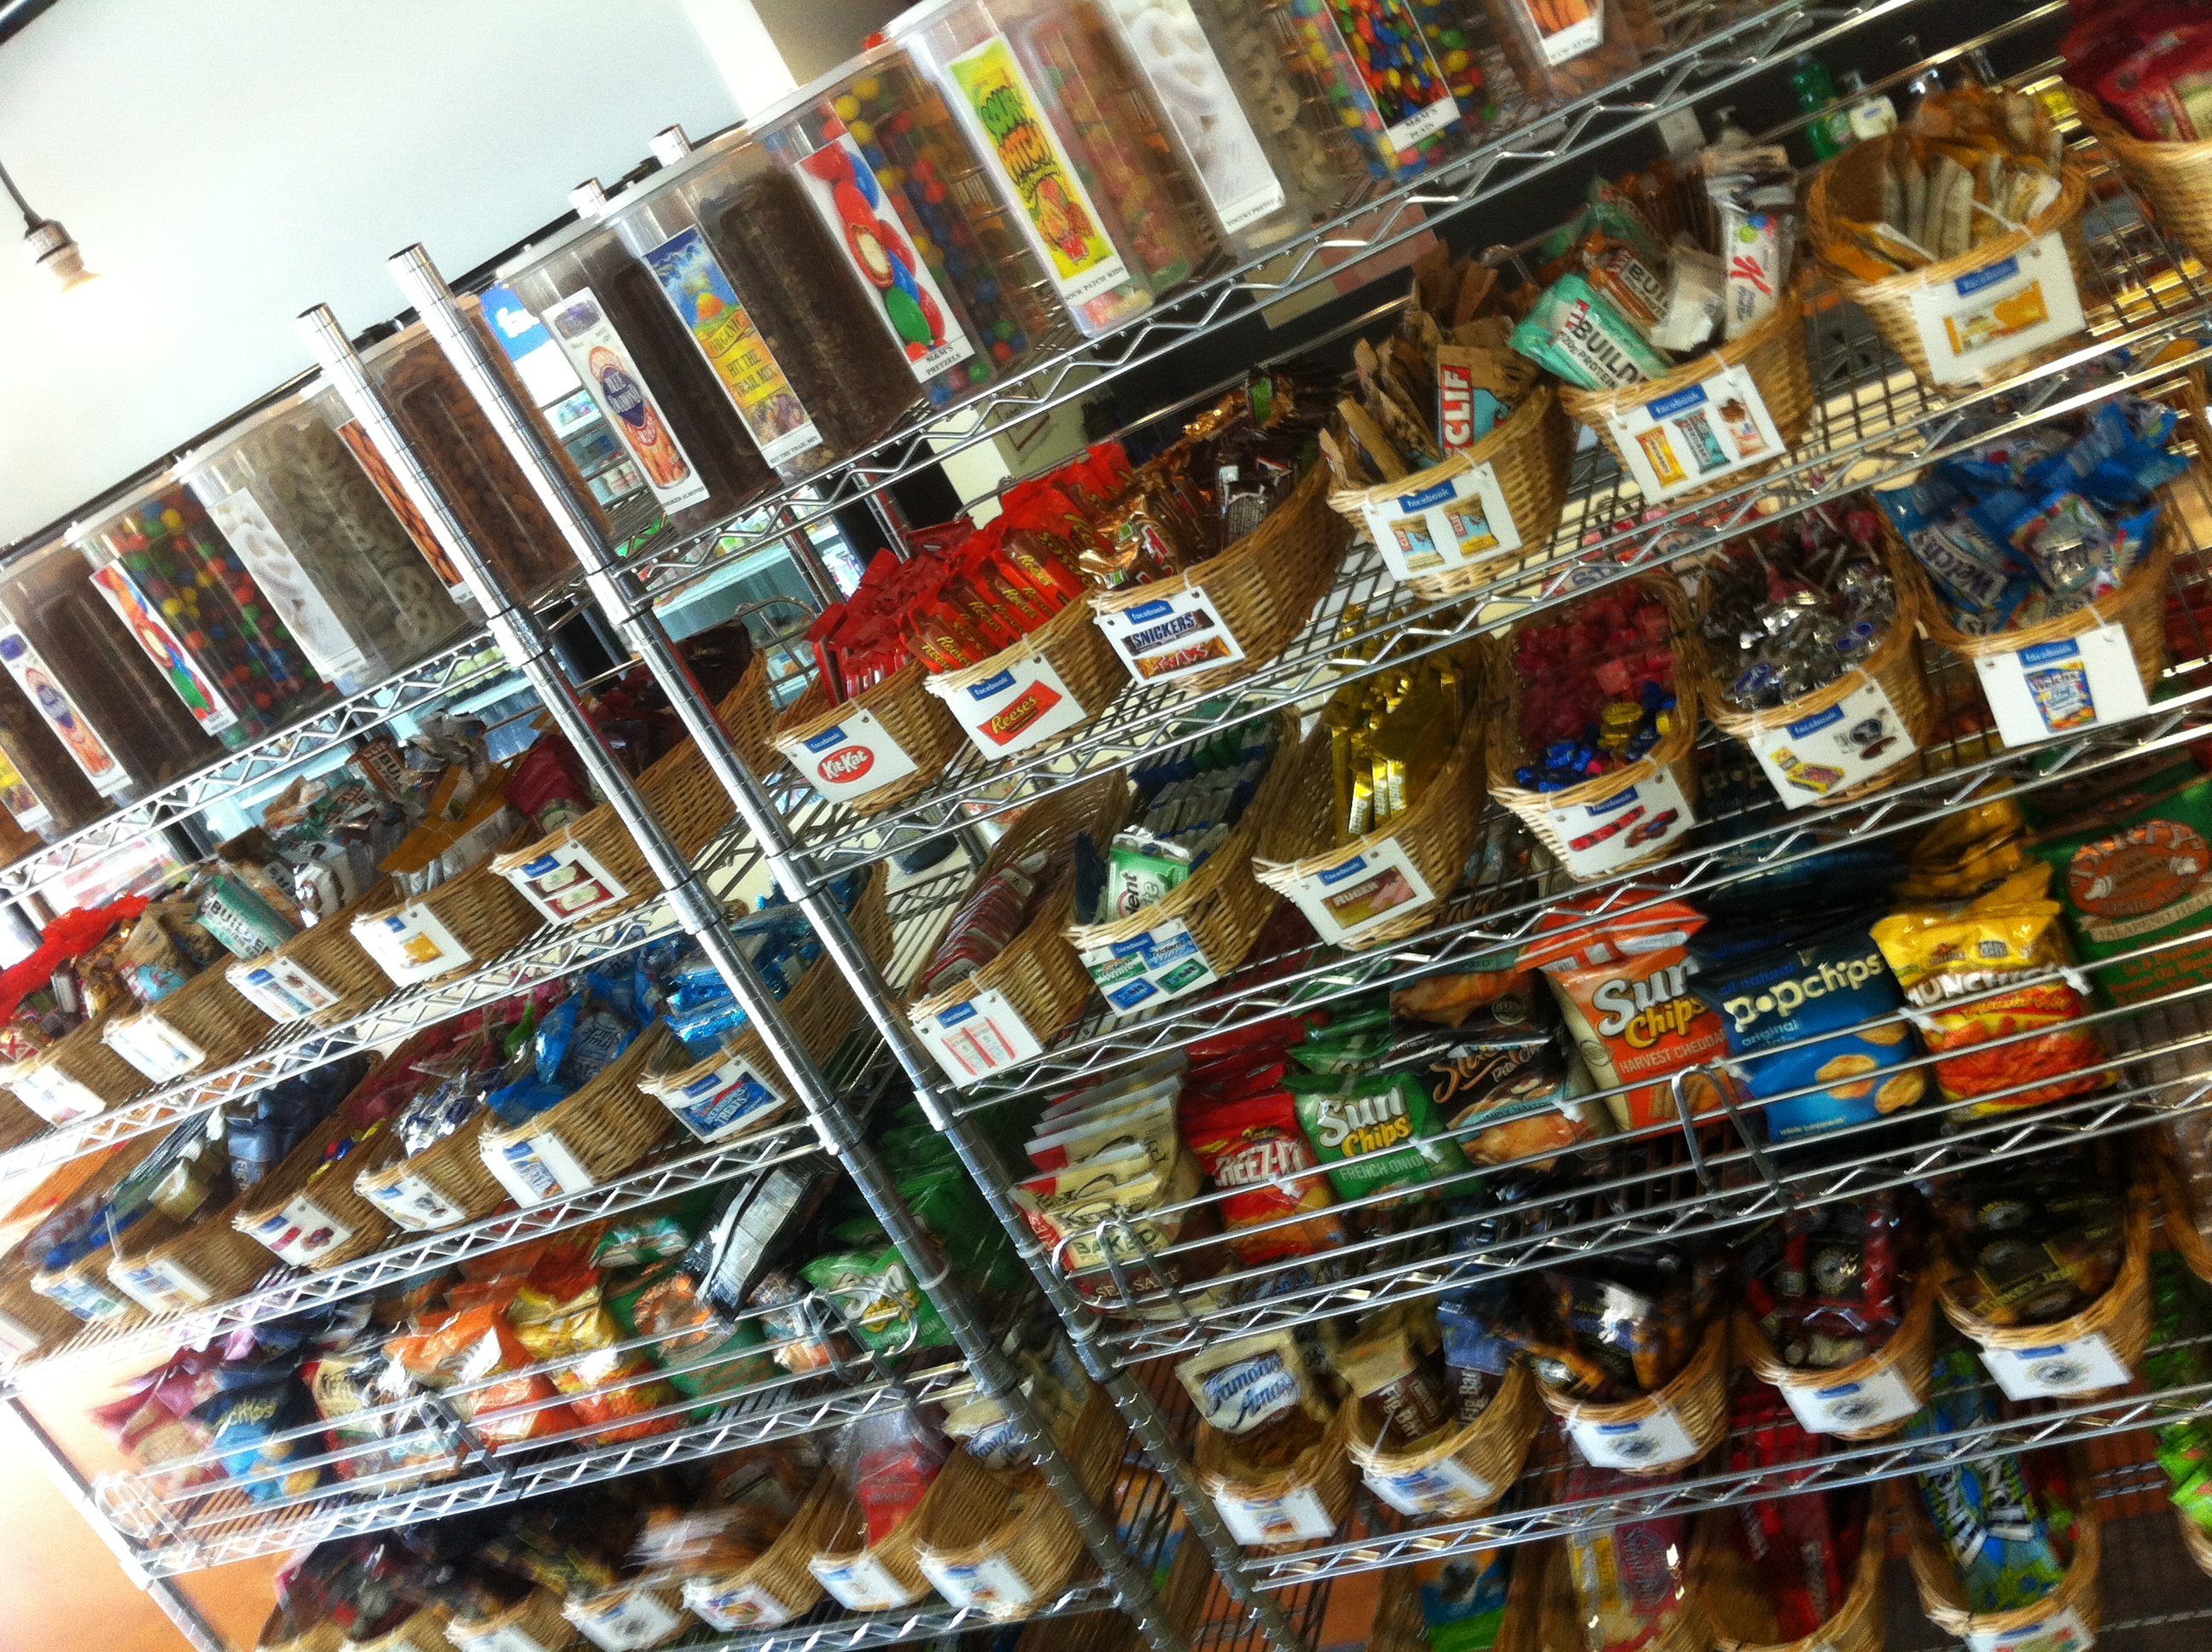
\includegraphics[width=.7\textwidth]{sntc/IMG_2050.JPG}
\end{center}
\end{block}
\end{frame}
\begin{frame}
\frametitle{Competições de Programação}
\begin{block}{Por que é Bom?}
\begin{center}
	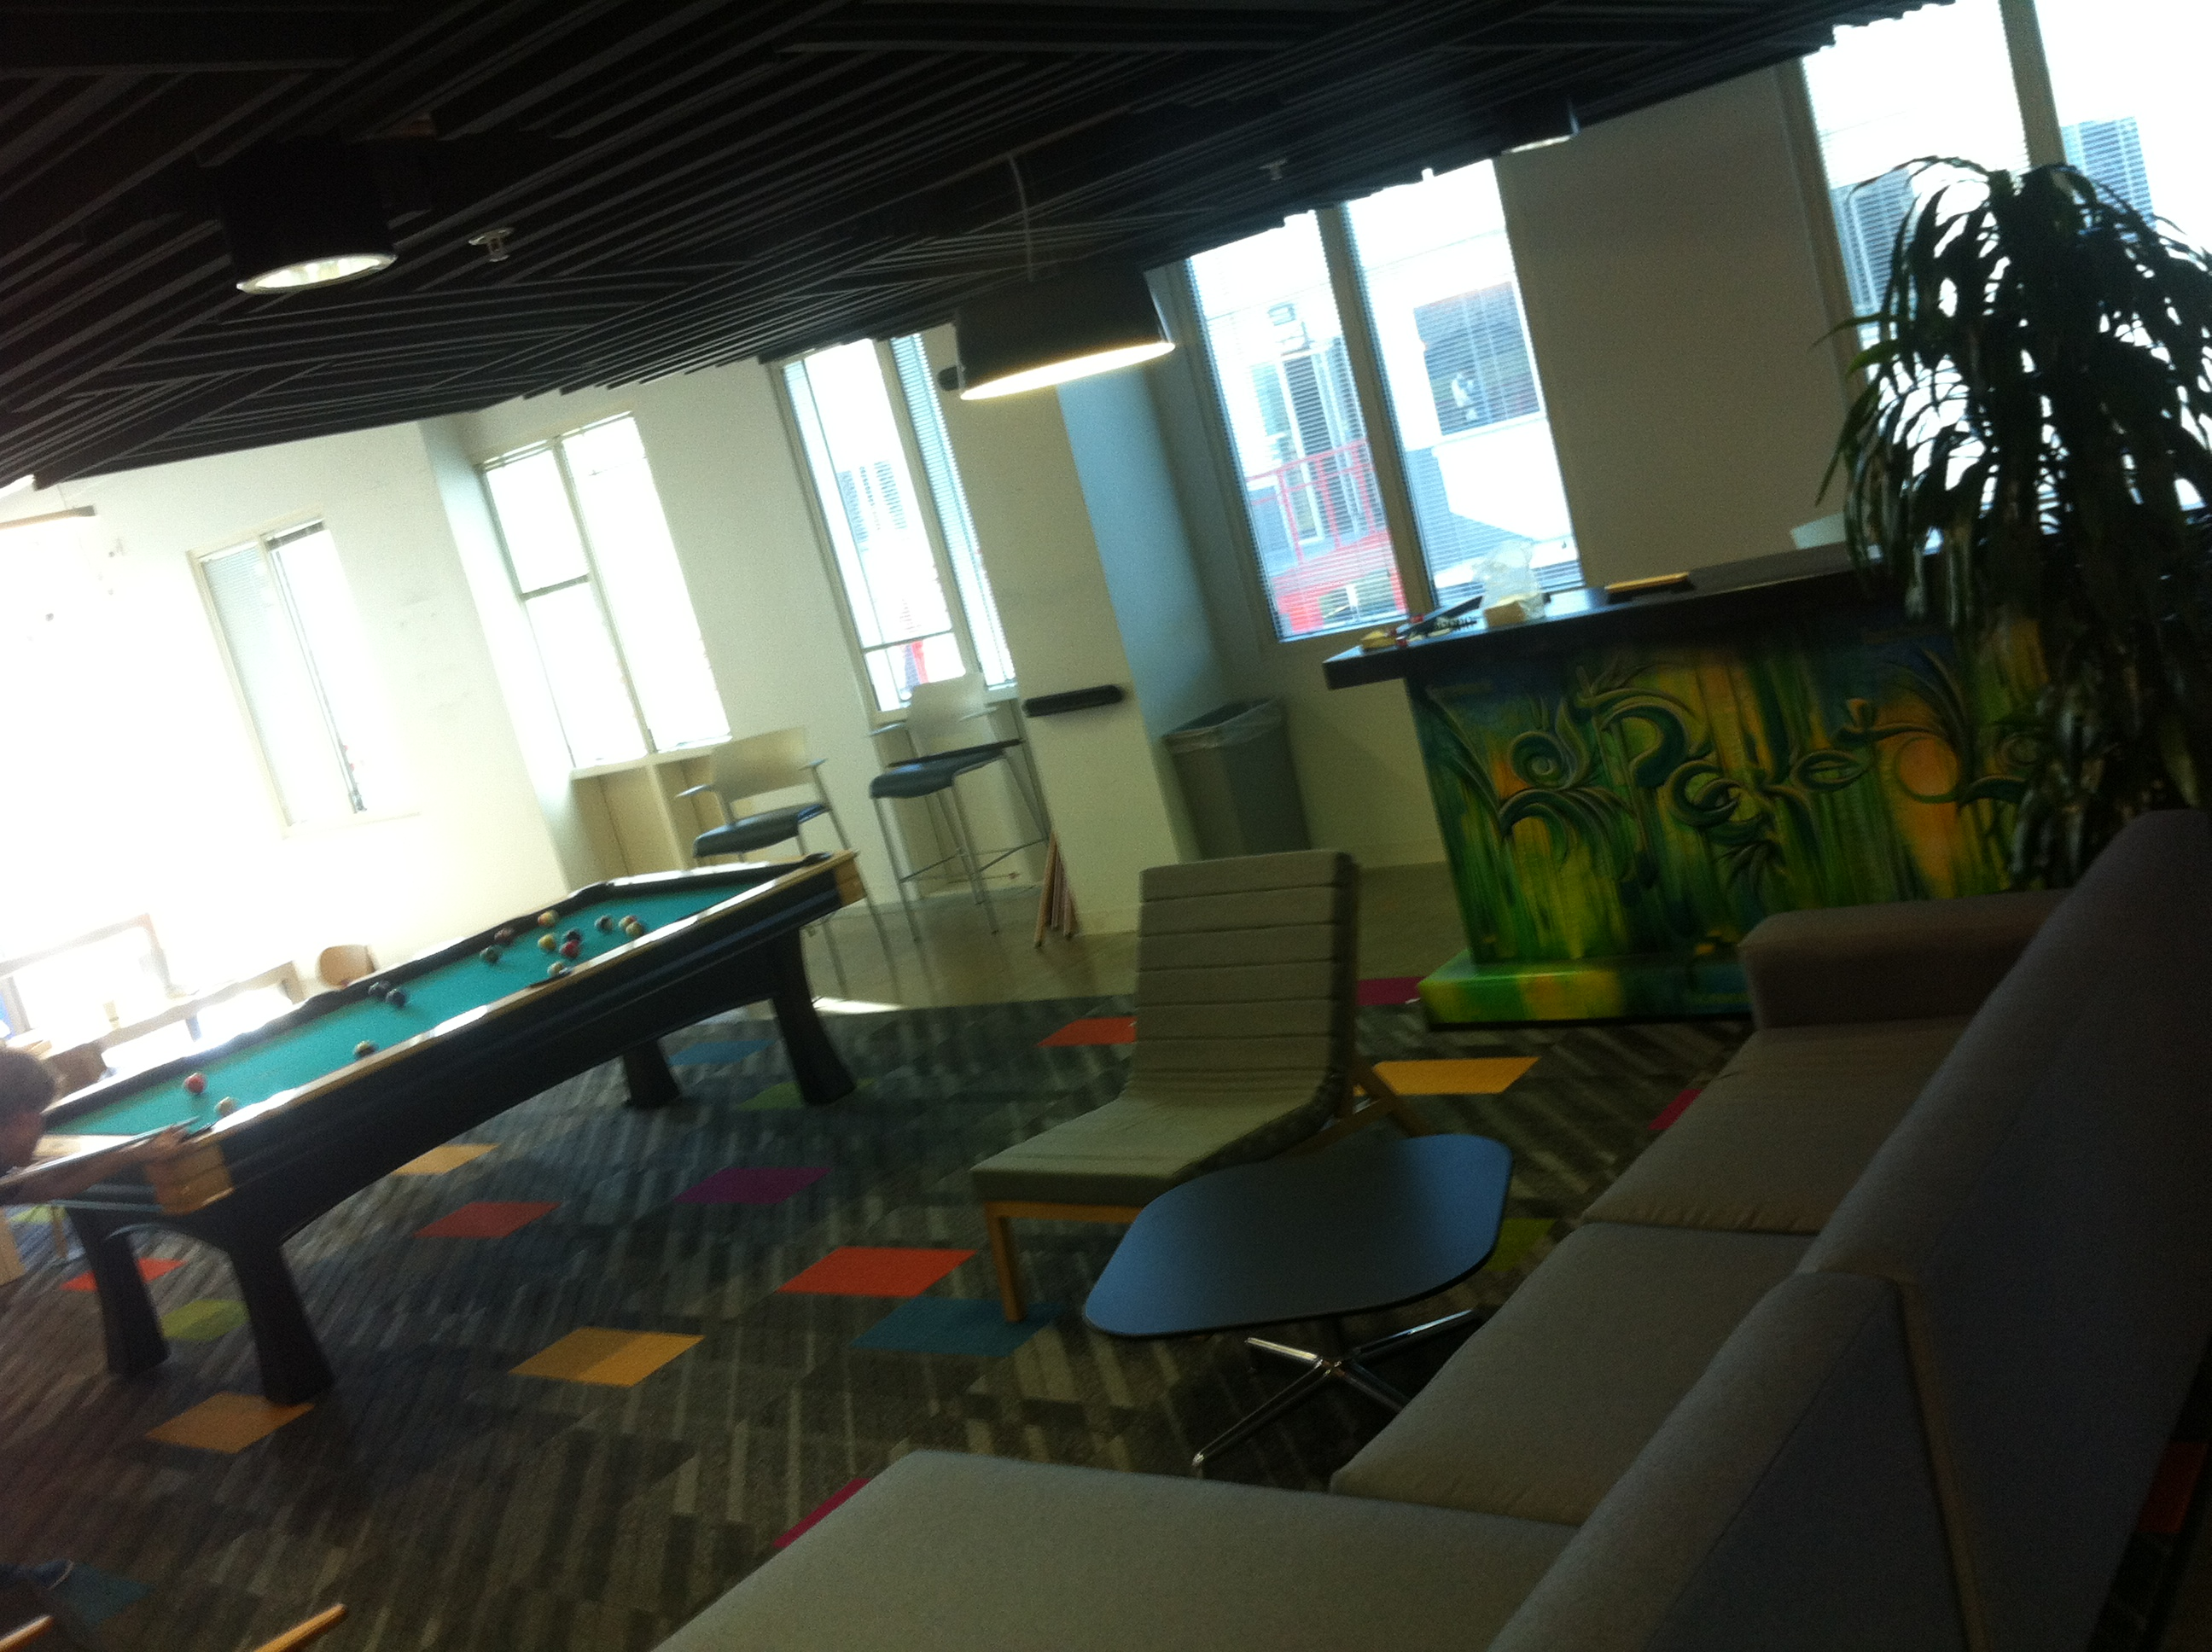
\includegraphics[width=.7\textwidth]{sntc/IMG_2051.JPG}
\end{center}
\end{block}
\end{frame}
\begin{frame}
\frametitle{Competições de Programação}
\begin{block}{Por que é Bom?}
\begin{center}
	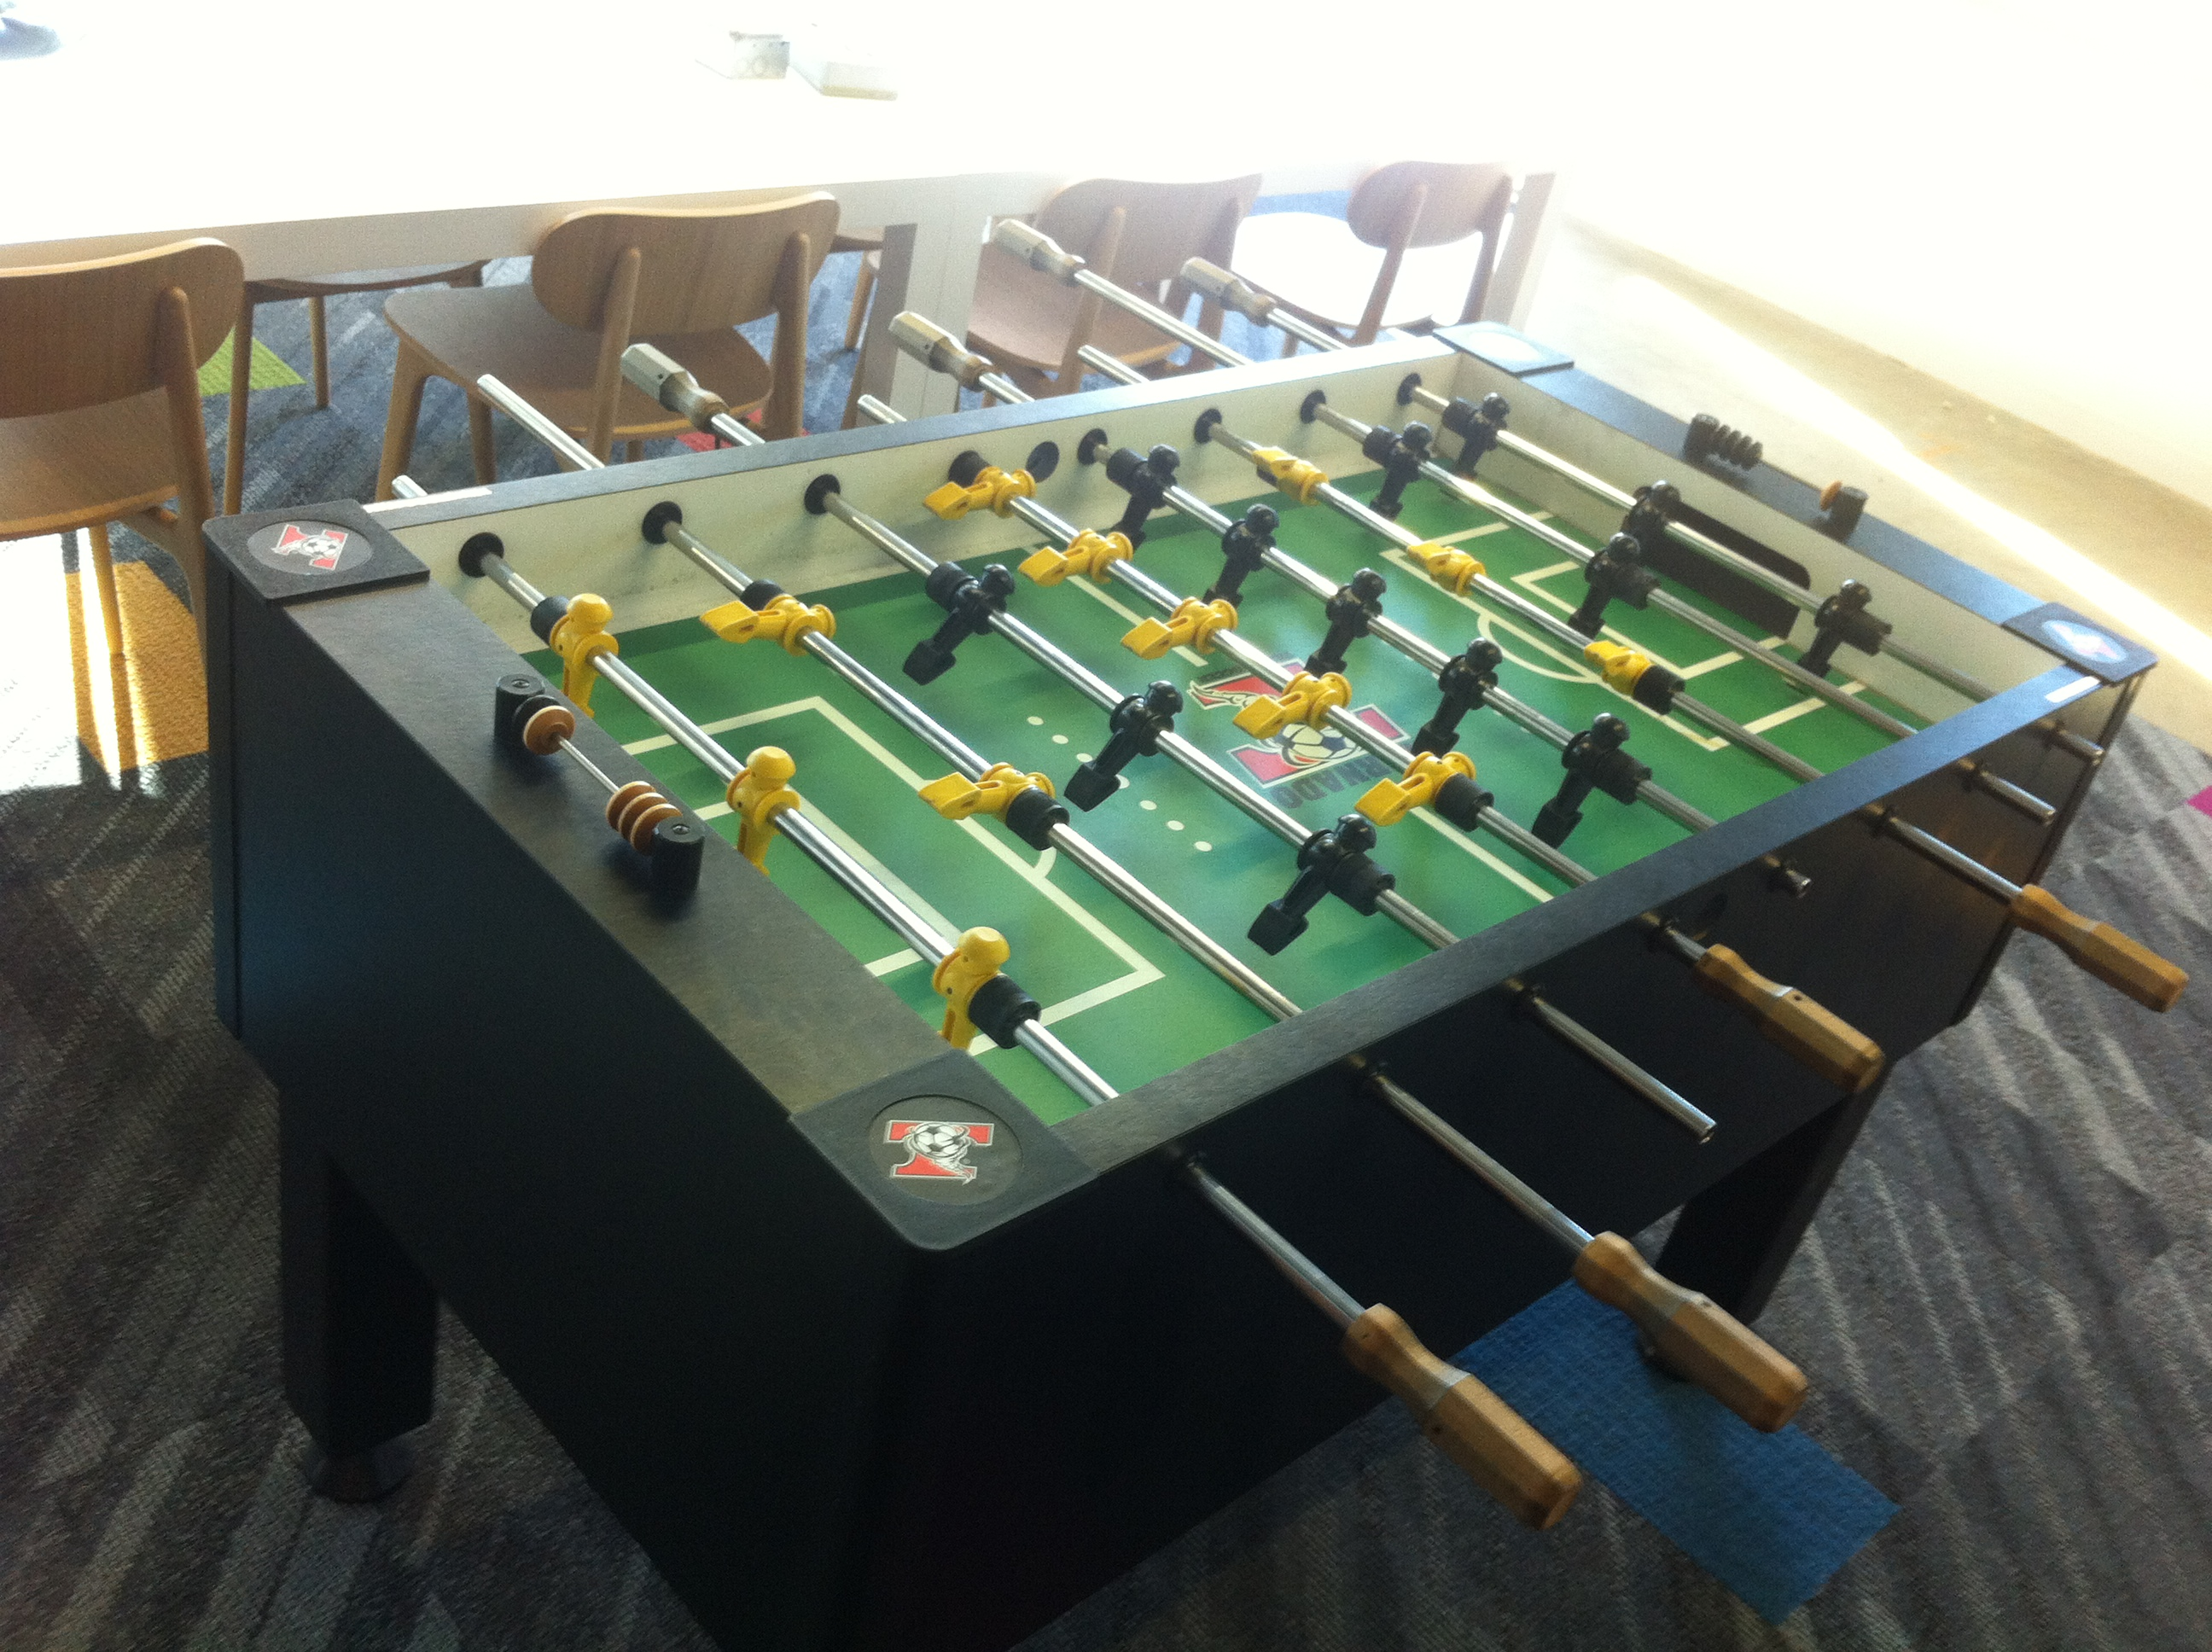
\includegraphics[width=.7\textwidth]{sntc/IMG_2052.JPG}
\end{center}
\end{block}
\end{frame}
\begin{frame}
\frametitle{Competições de Programação}
\begin{block}{Por que é Bom?}
\begin{center}
	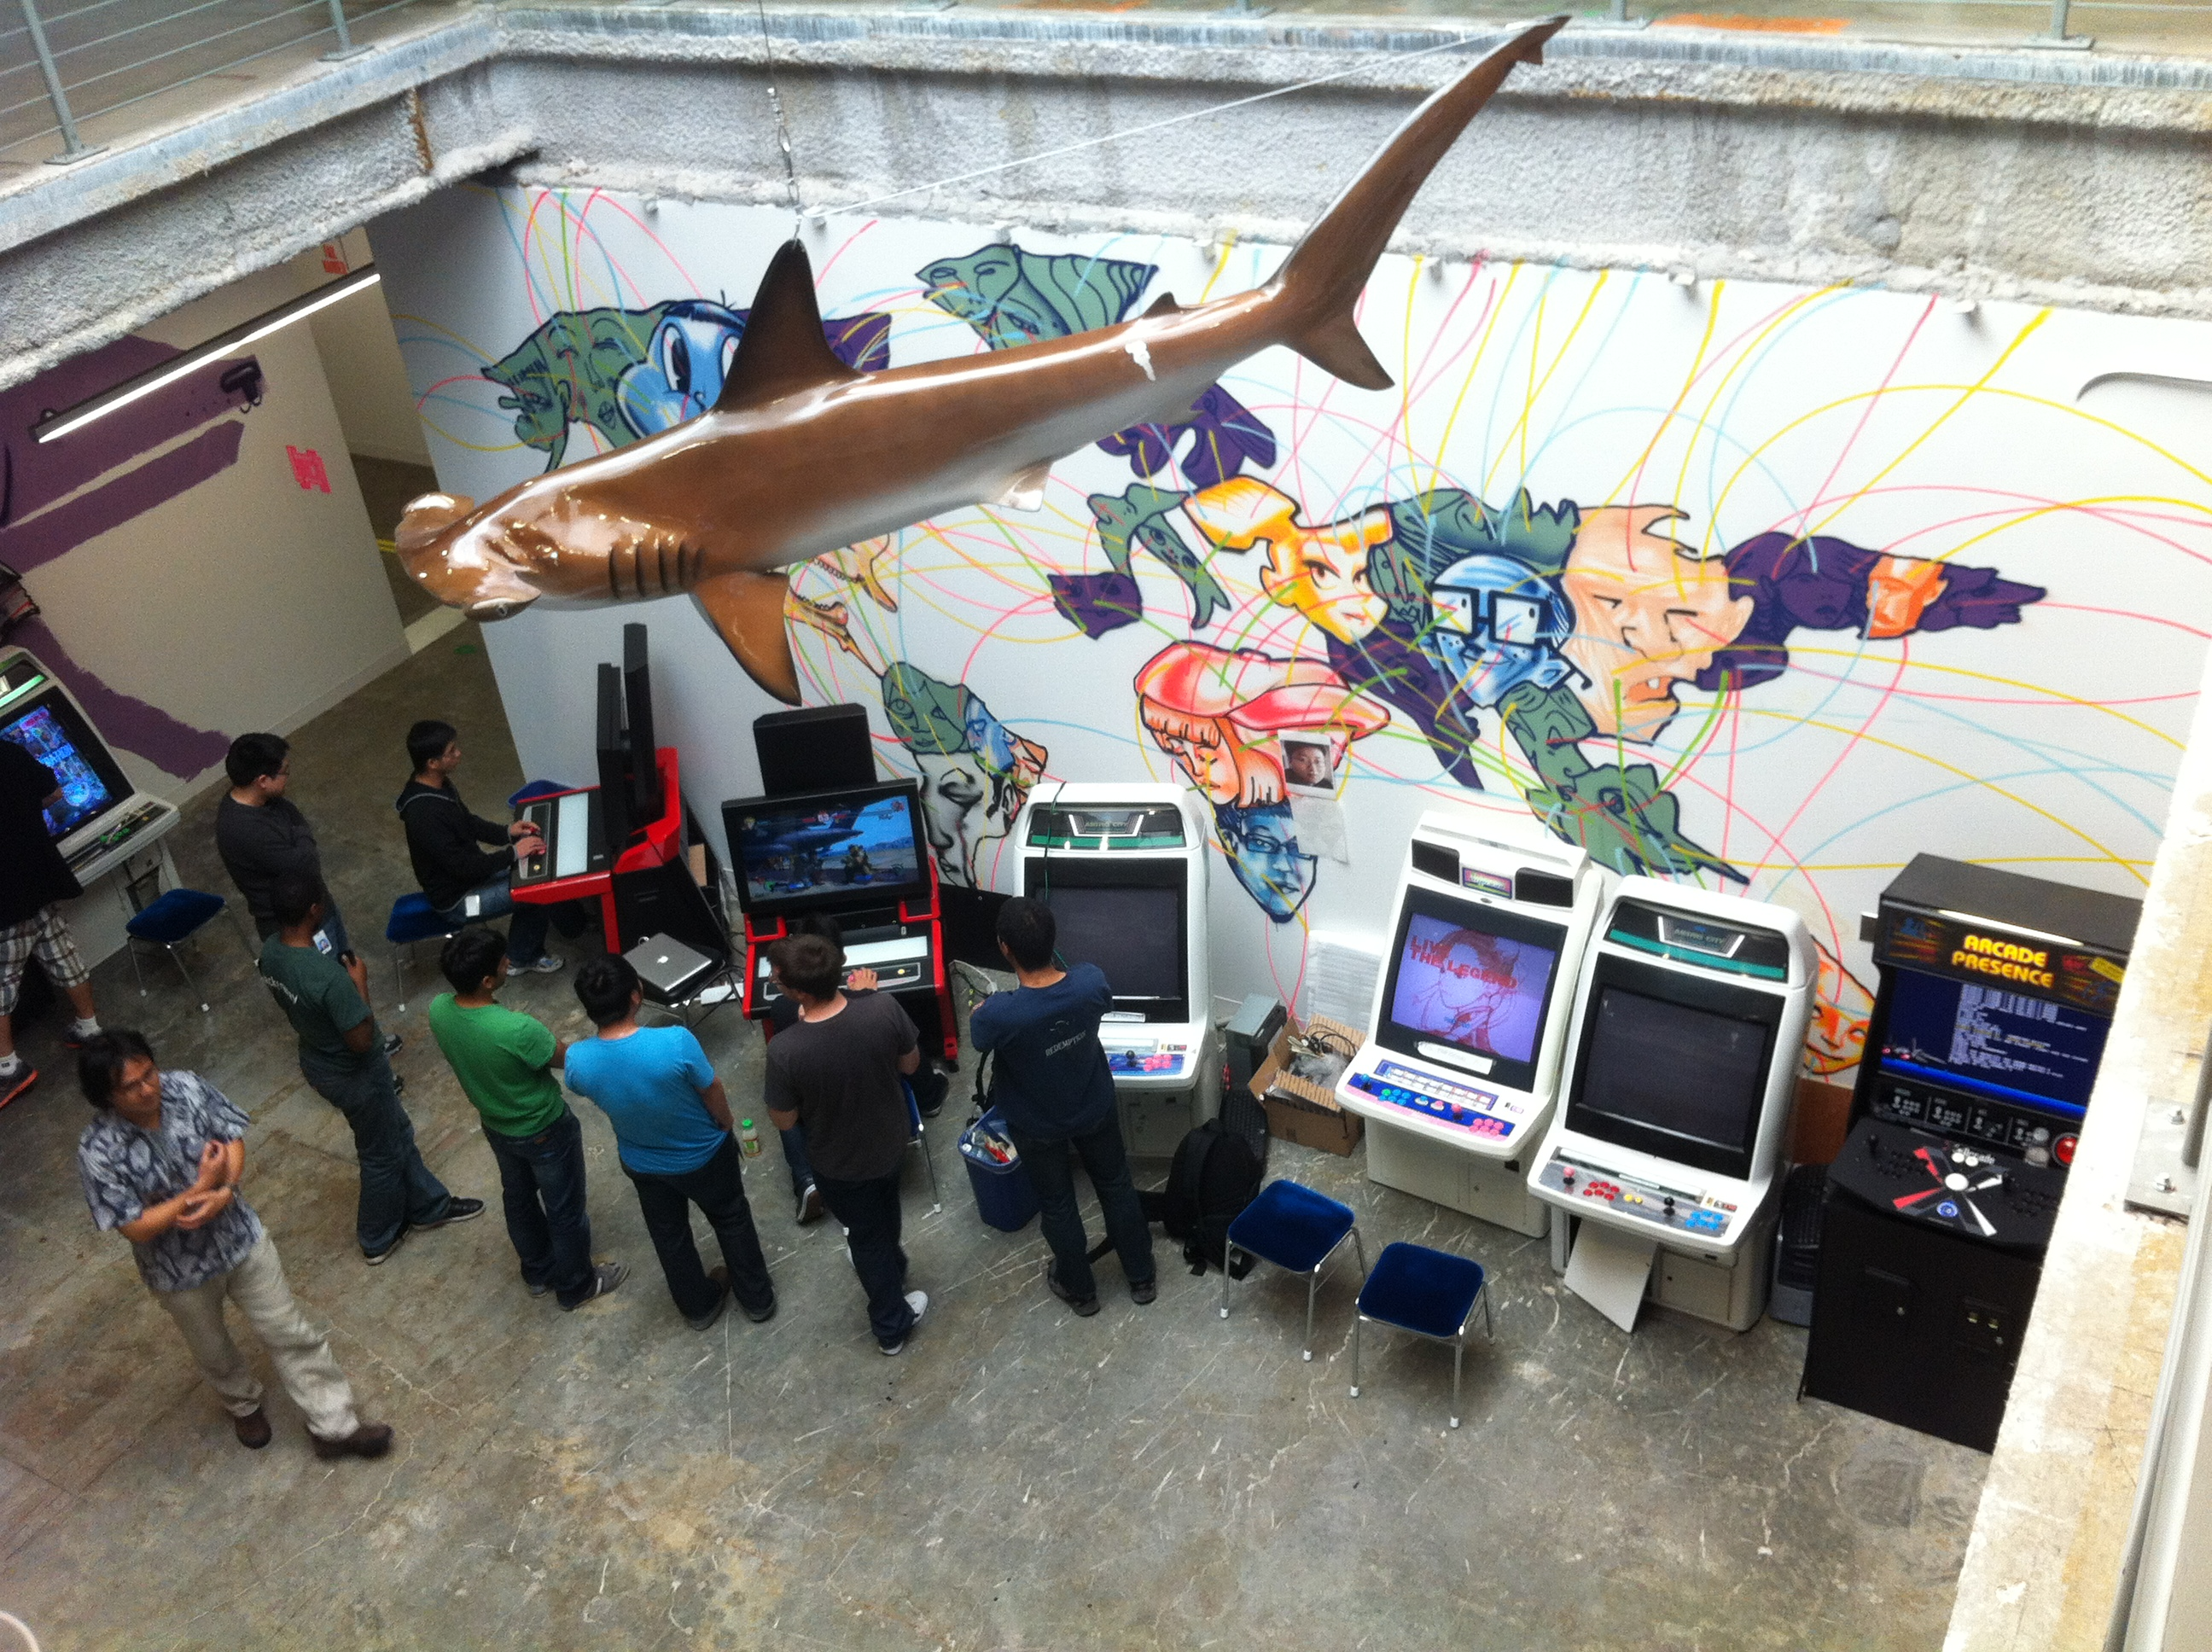
\includegraphics[width=.7\textwidth]{sntc/IMG_2056.JPG}
\end{center}
\end{block}
\end{frame}
\begin{frame}
\frametitle{Competições de Programação}
\begin{block}{Por que é Bom?}
\begin{center}
	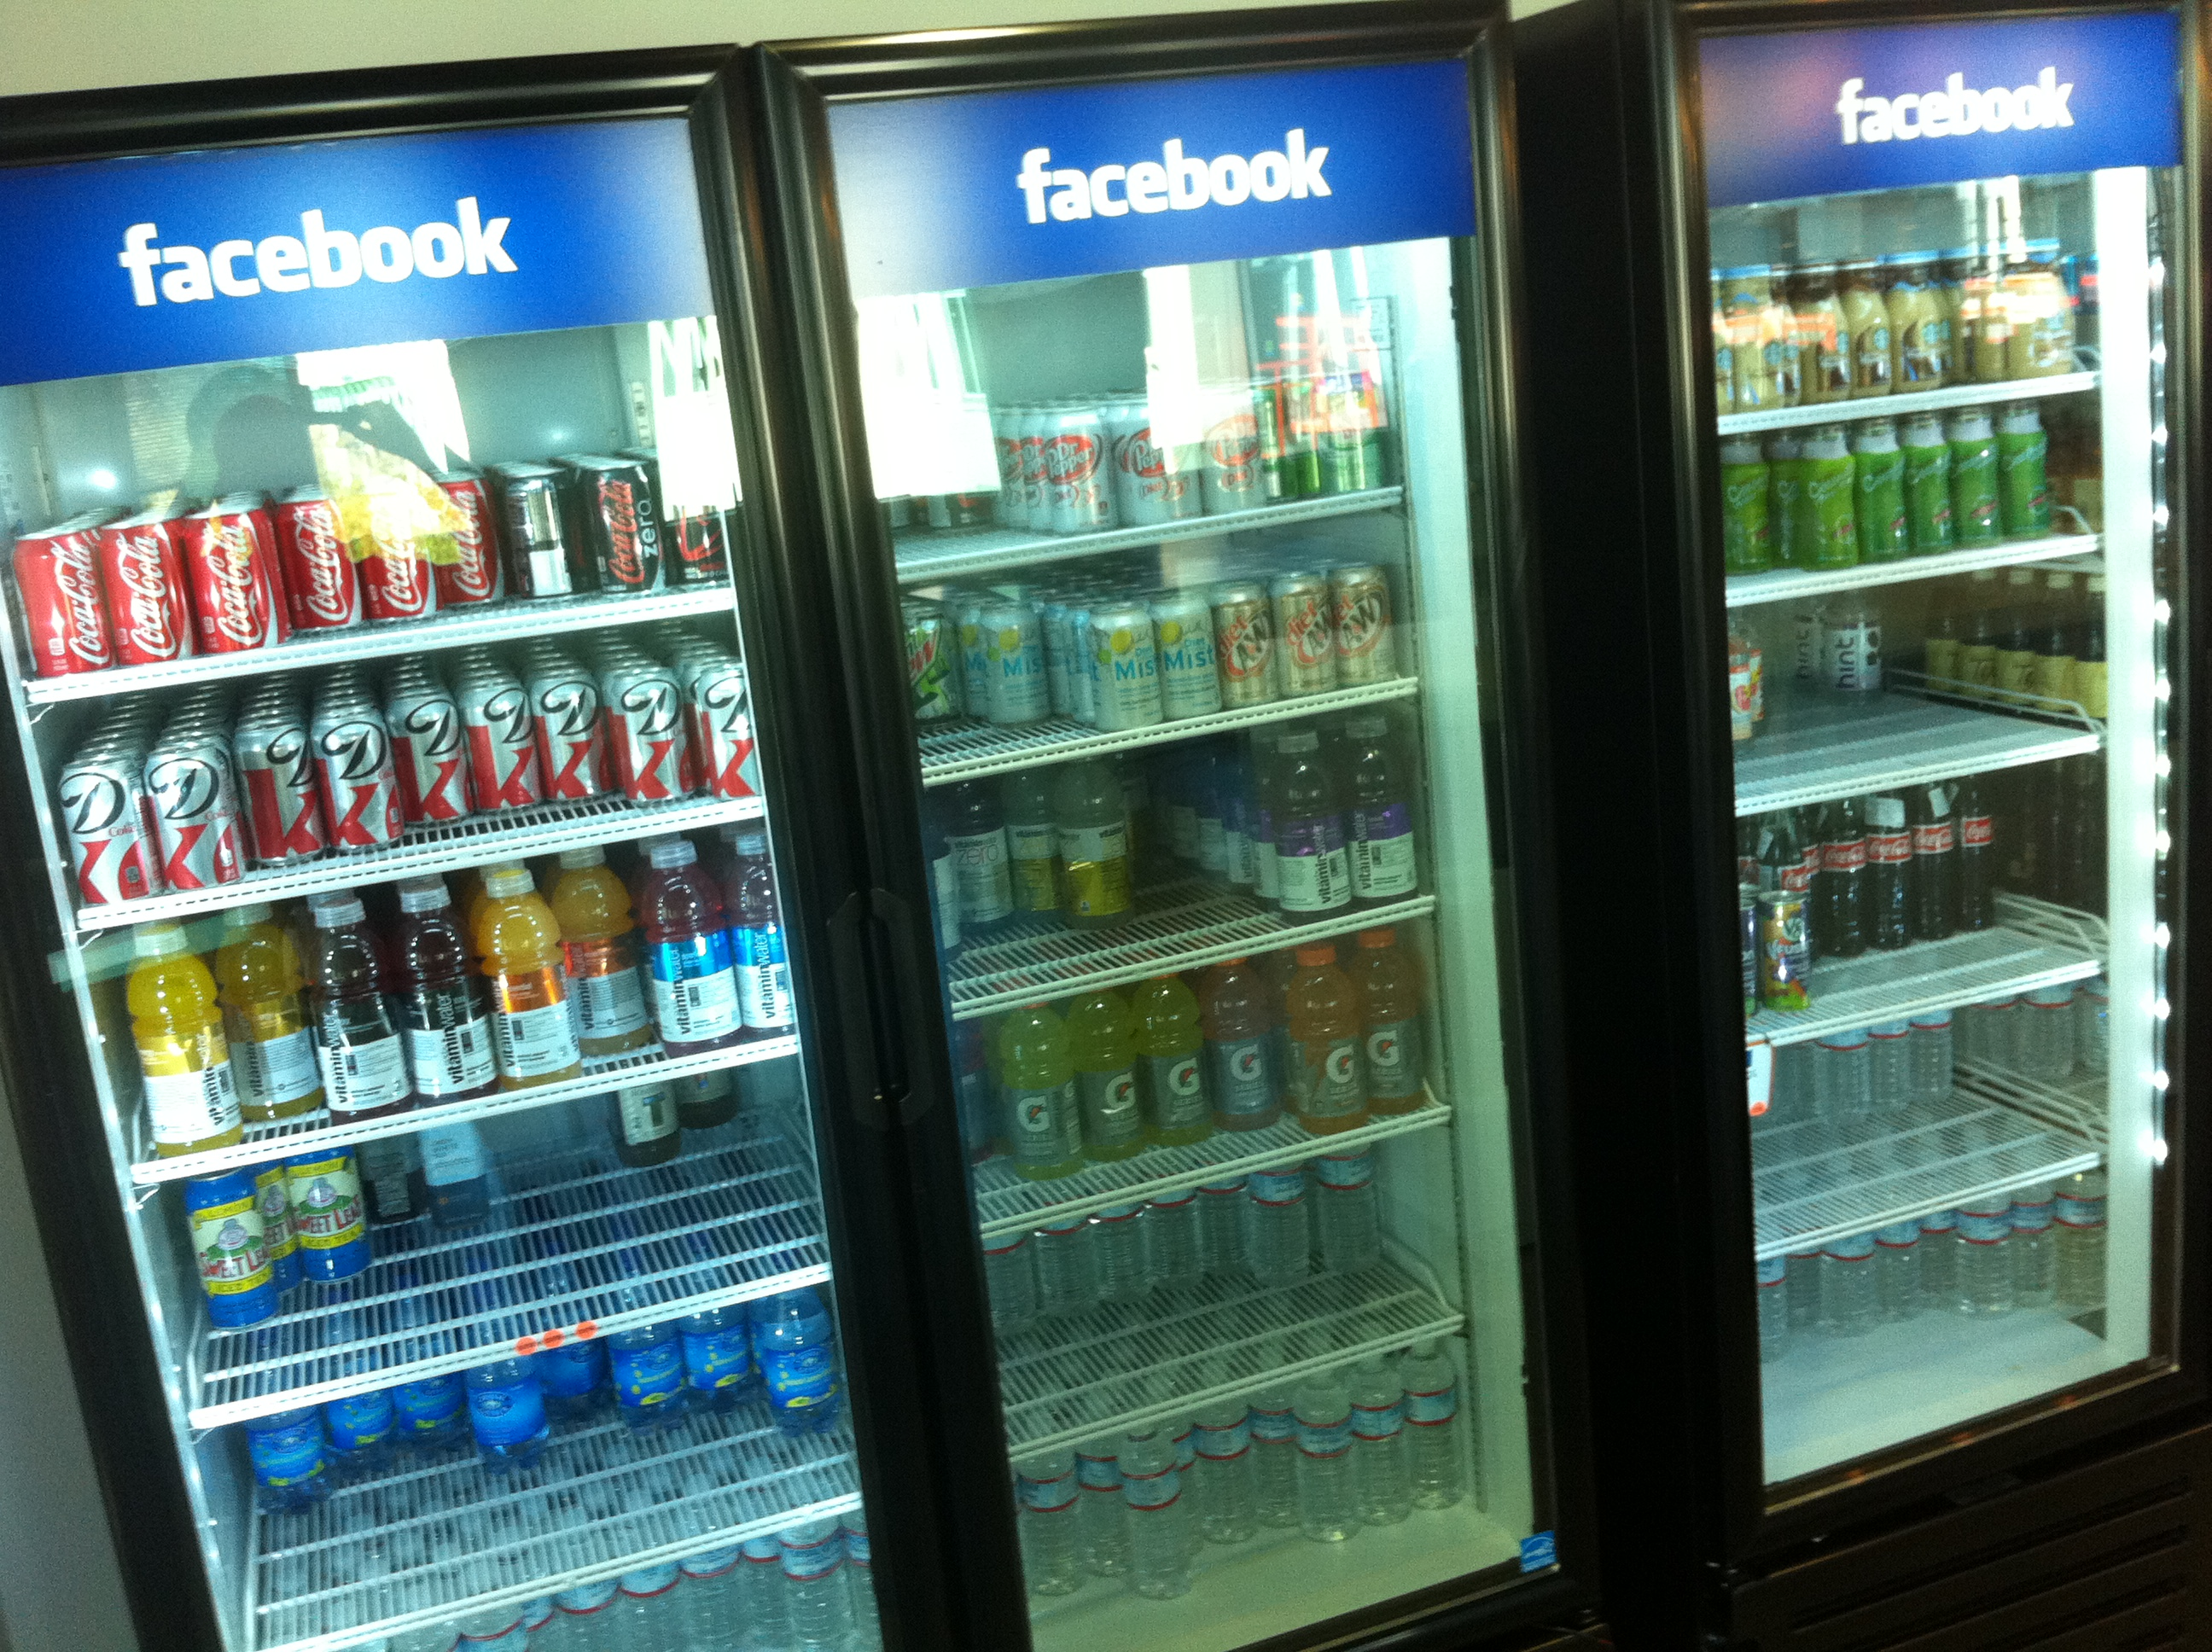
\includegraphics[width=.7\textwidth]{sntc/IMG_2062.JPG}
\end{center}
\end{block}
\end{frame}
\begin{frame}
\frametitle{Competições de Programação}
\begin{block}{Por que é Bom?}
\begin{center}
	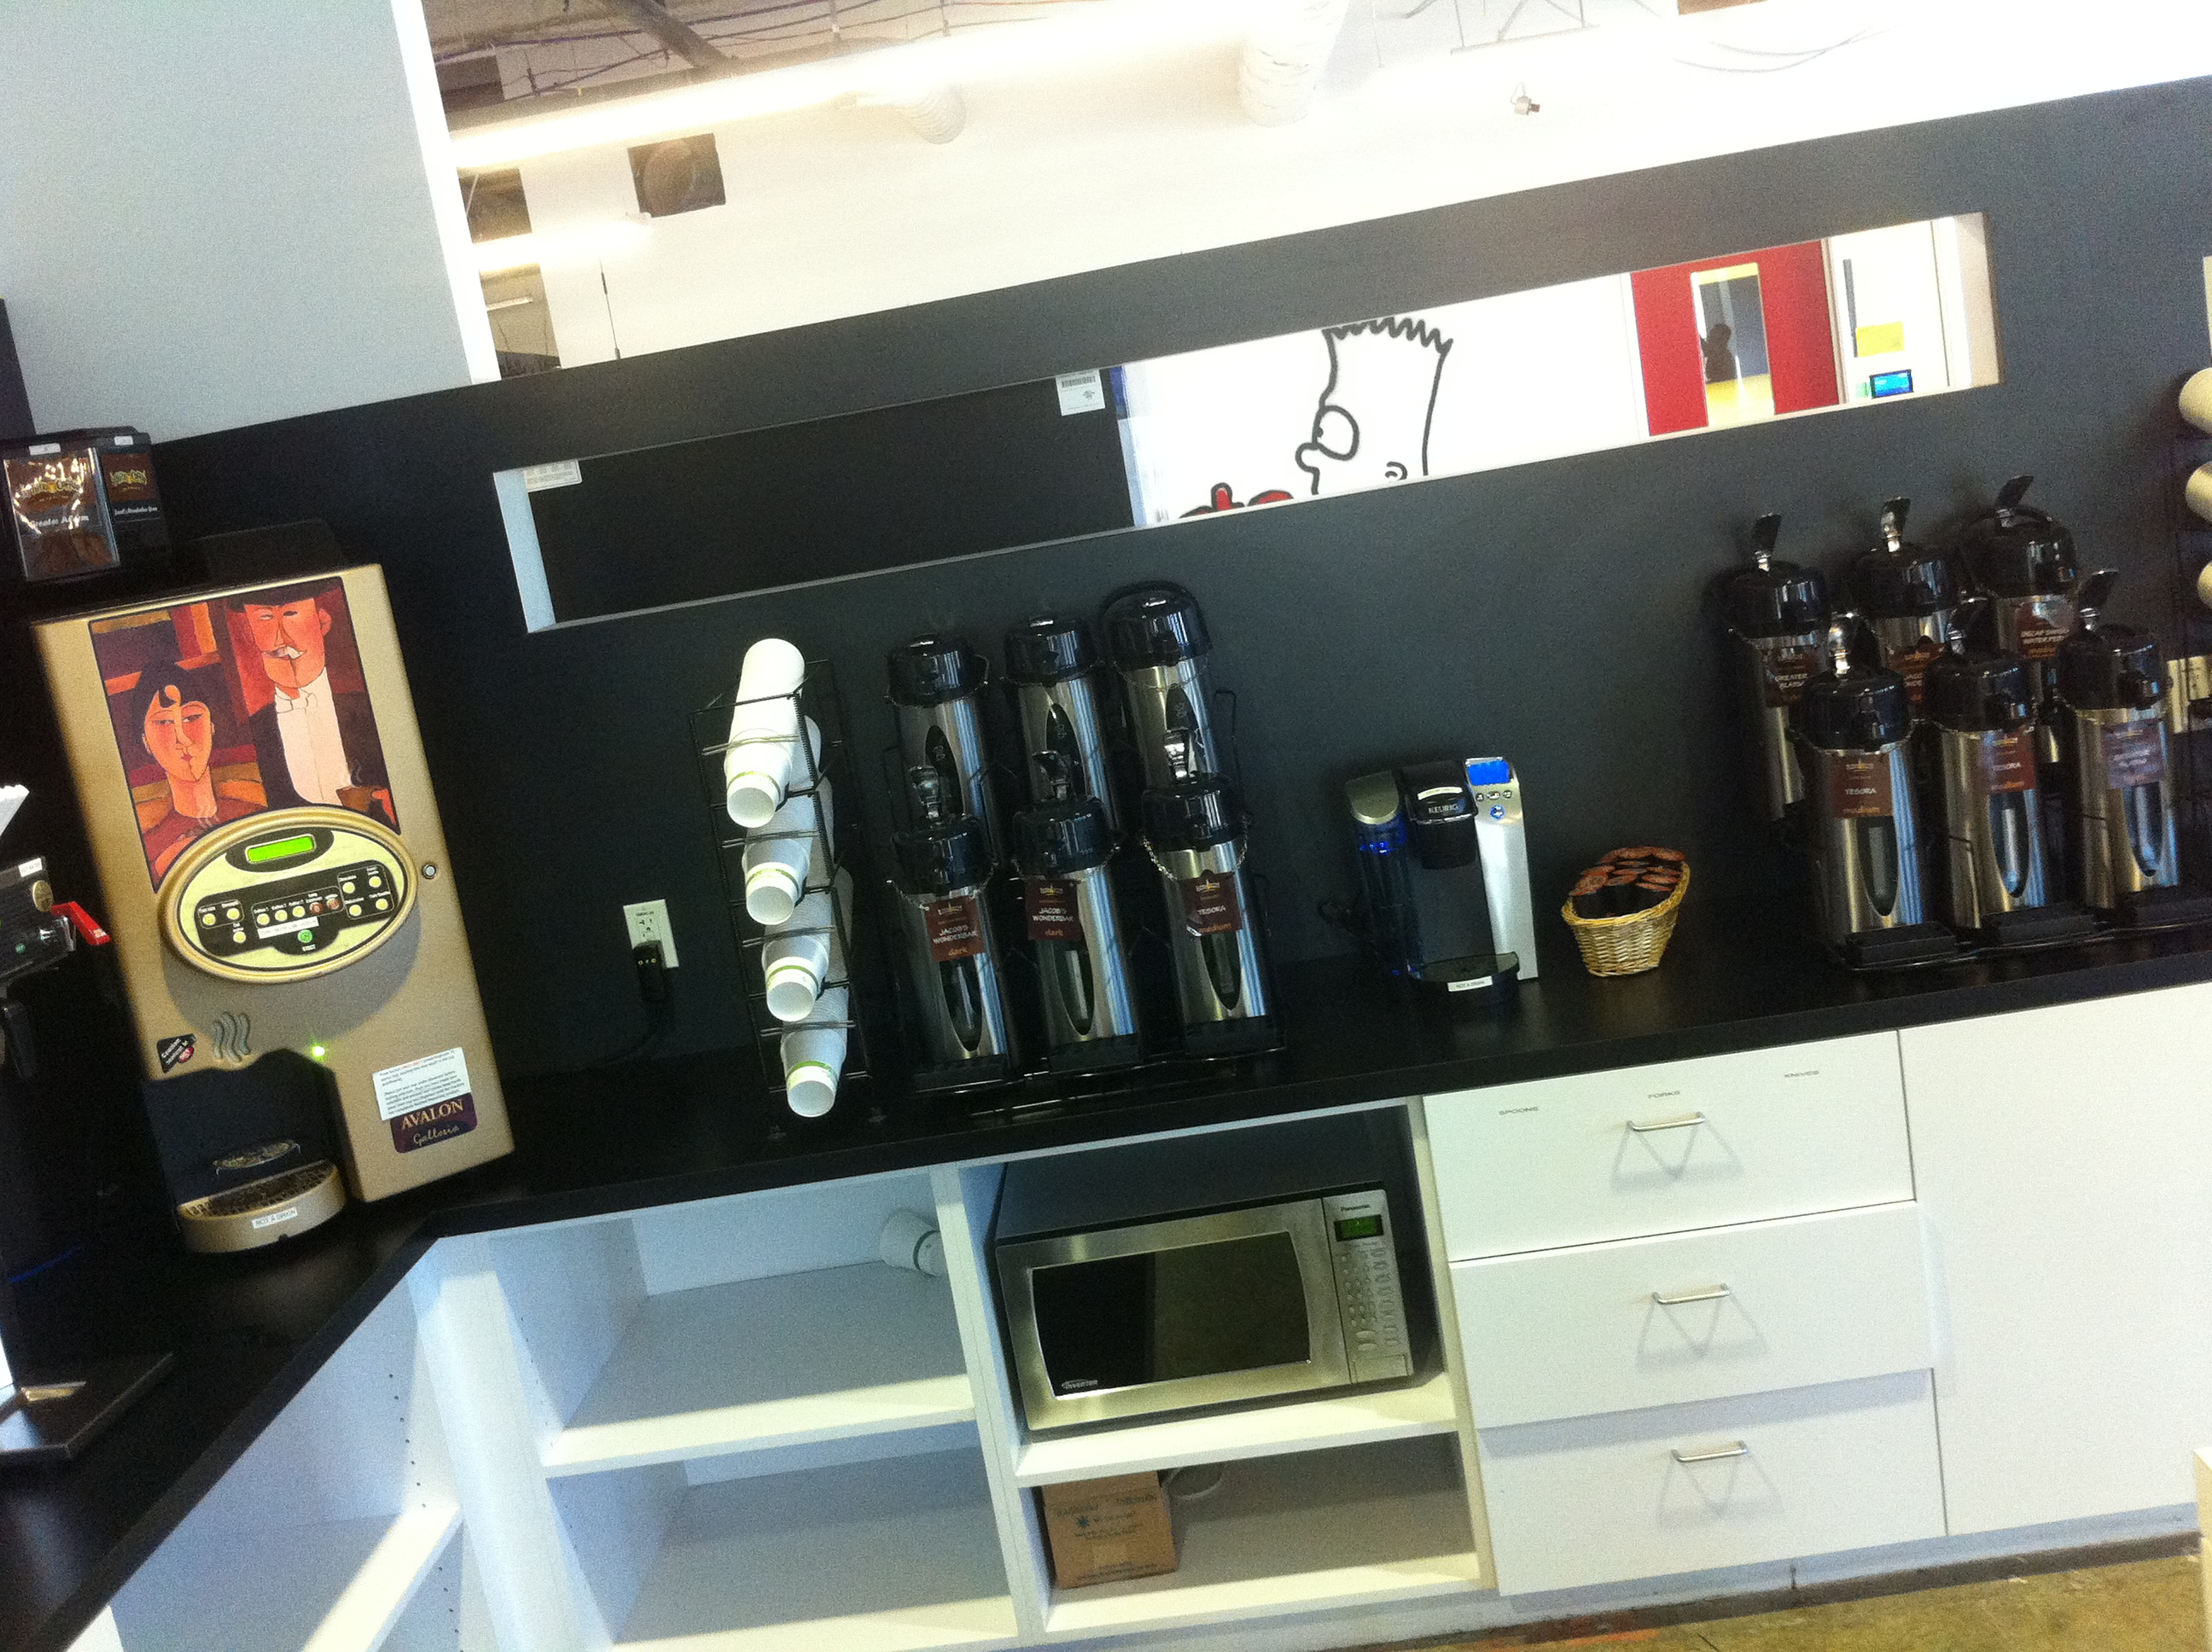
\includegraphics[width=.7\textwidth]{sntc/IMG_2064.JPG}
\end{center}
\end{block}
\end{frame}
\begin{frame}
\frametitle{Competições de Programação}
\begin{block}{Por que é Bom?}
\begin{center}
	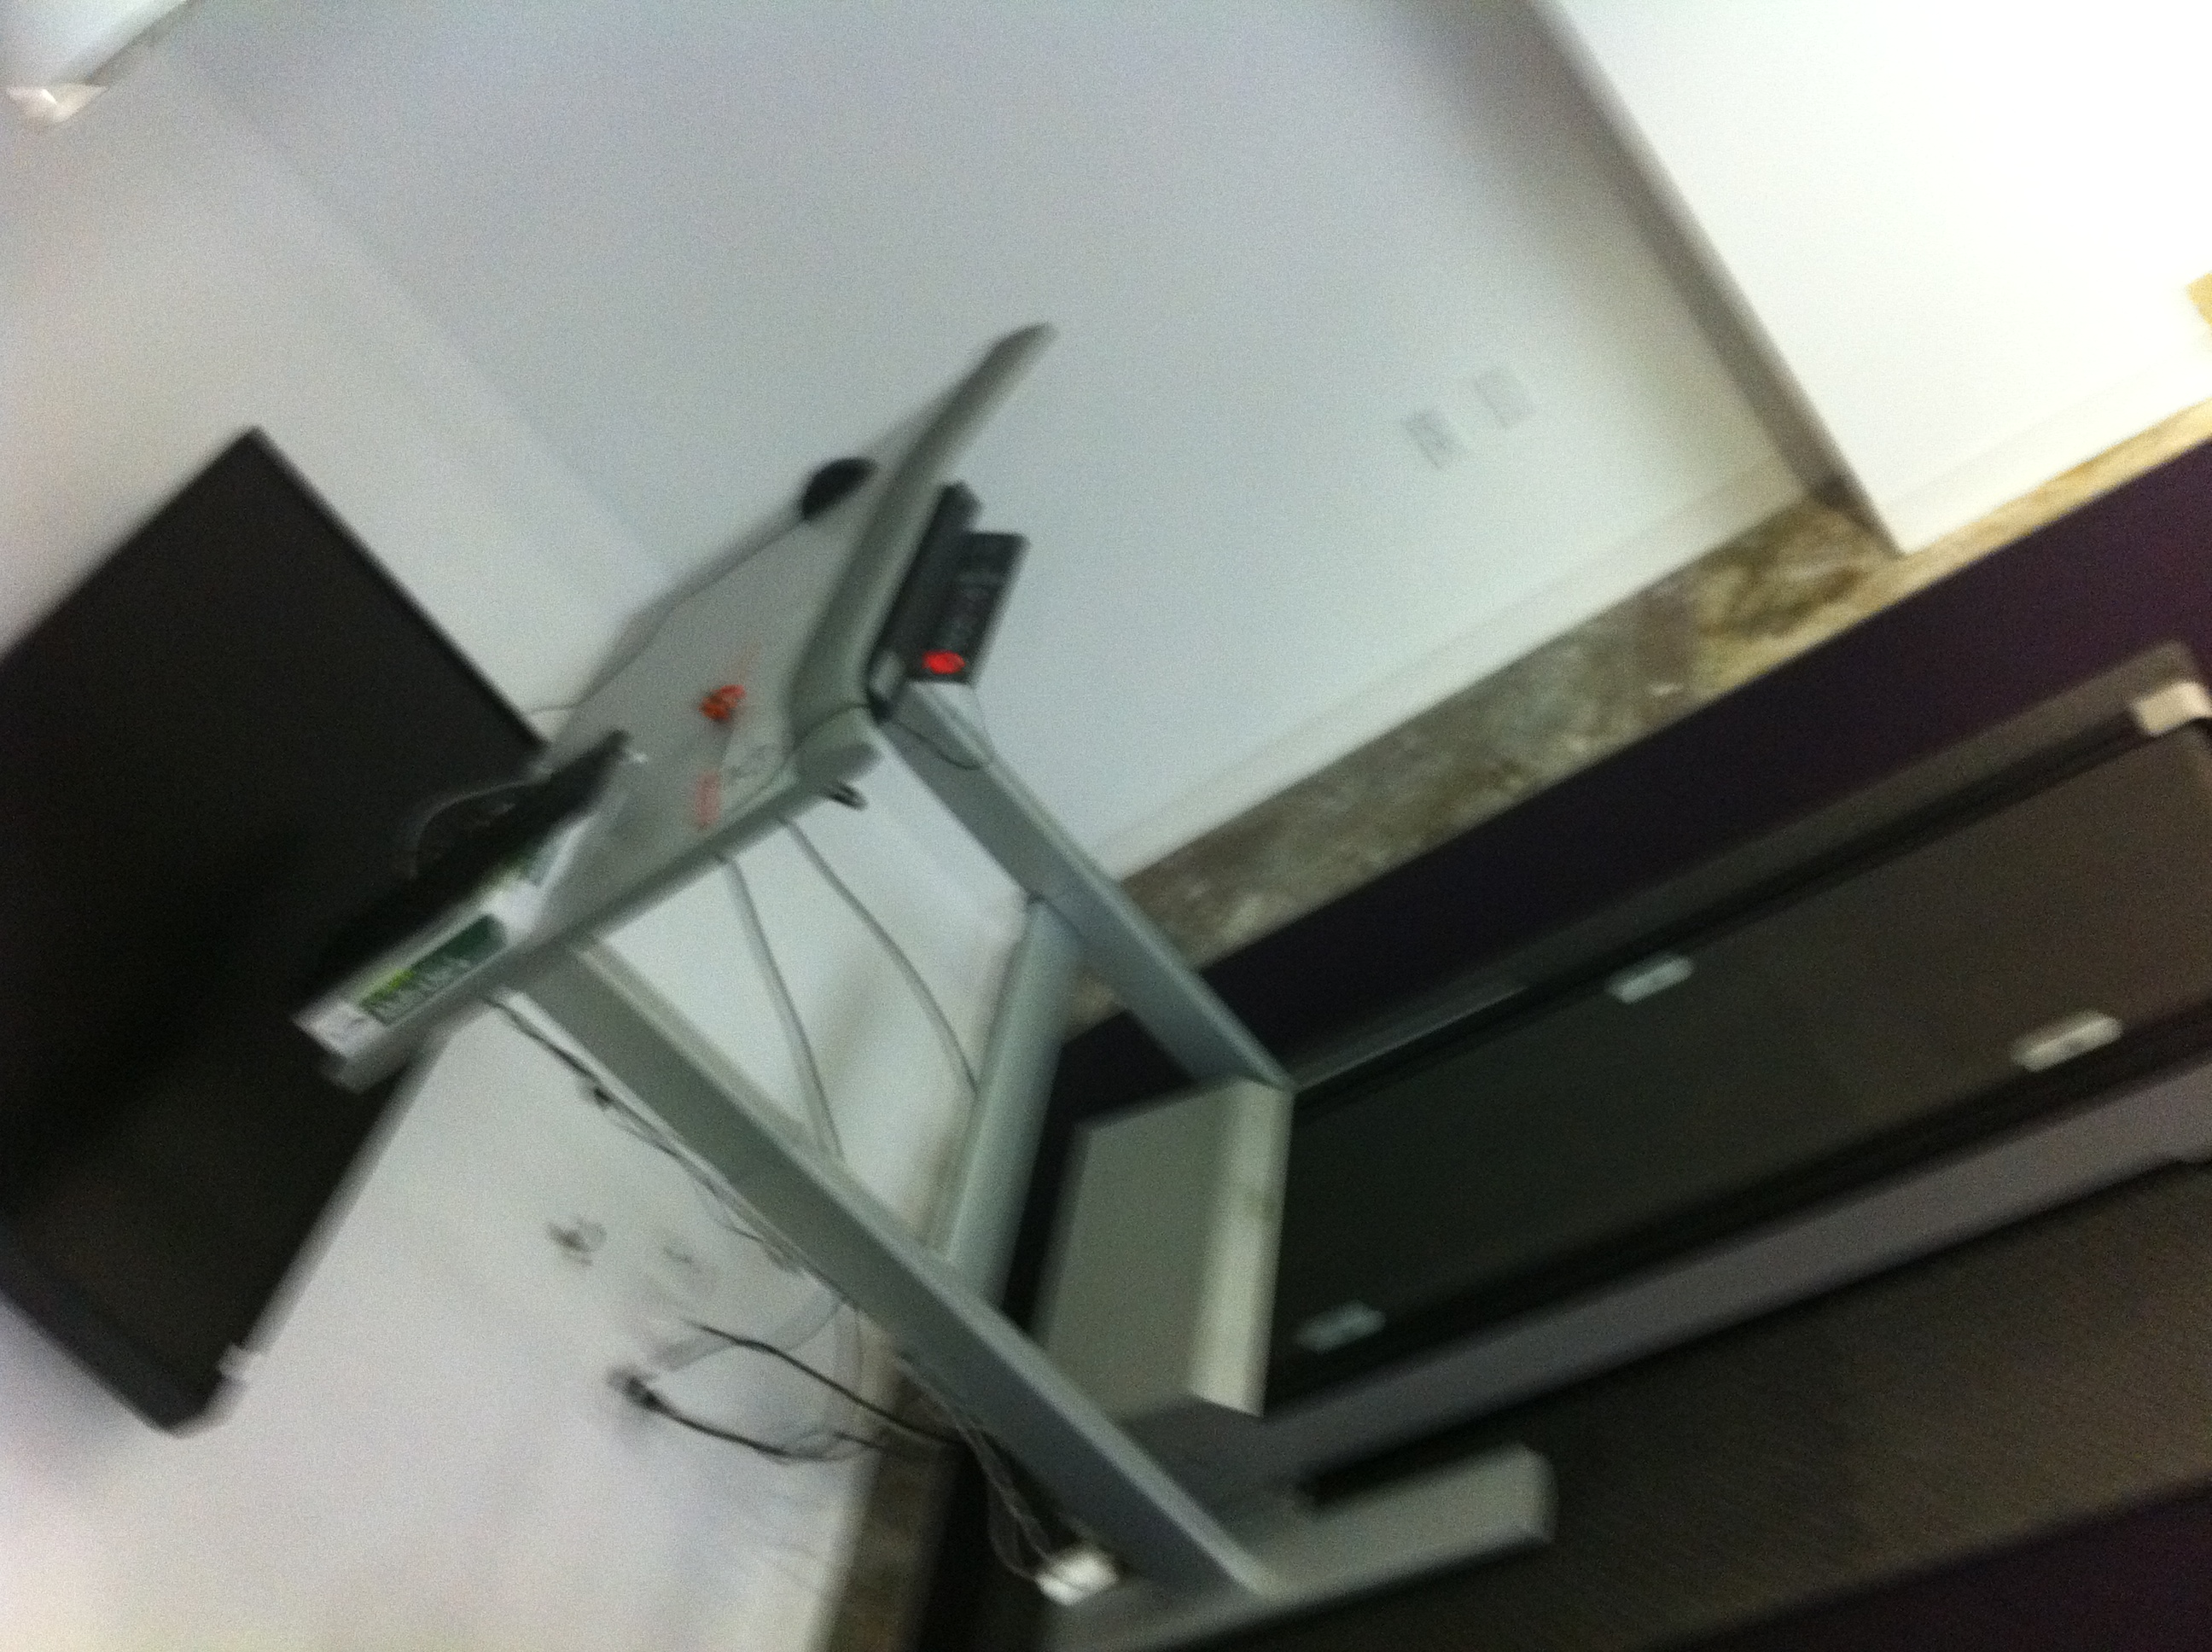
\includegraphics[width=.7\textwidth]{sntc/IMG_2066.JPG}
\end{center}
\end{block}
\end{frame}
\begin{frame}
\frametitle{Competições de Programação}
\begin{block}{Por que é Bom?}
\begin{center}
	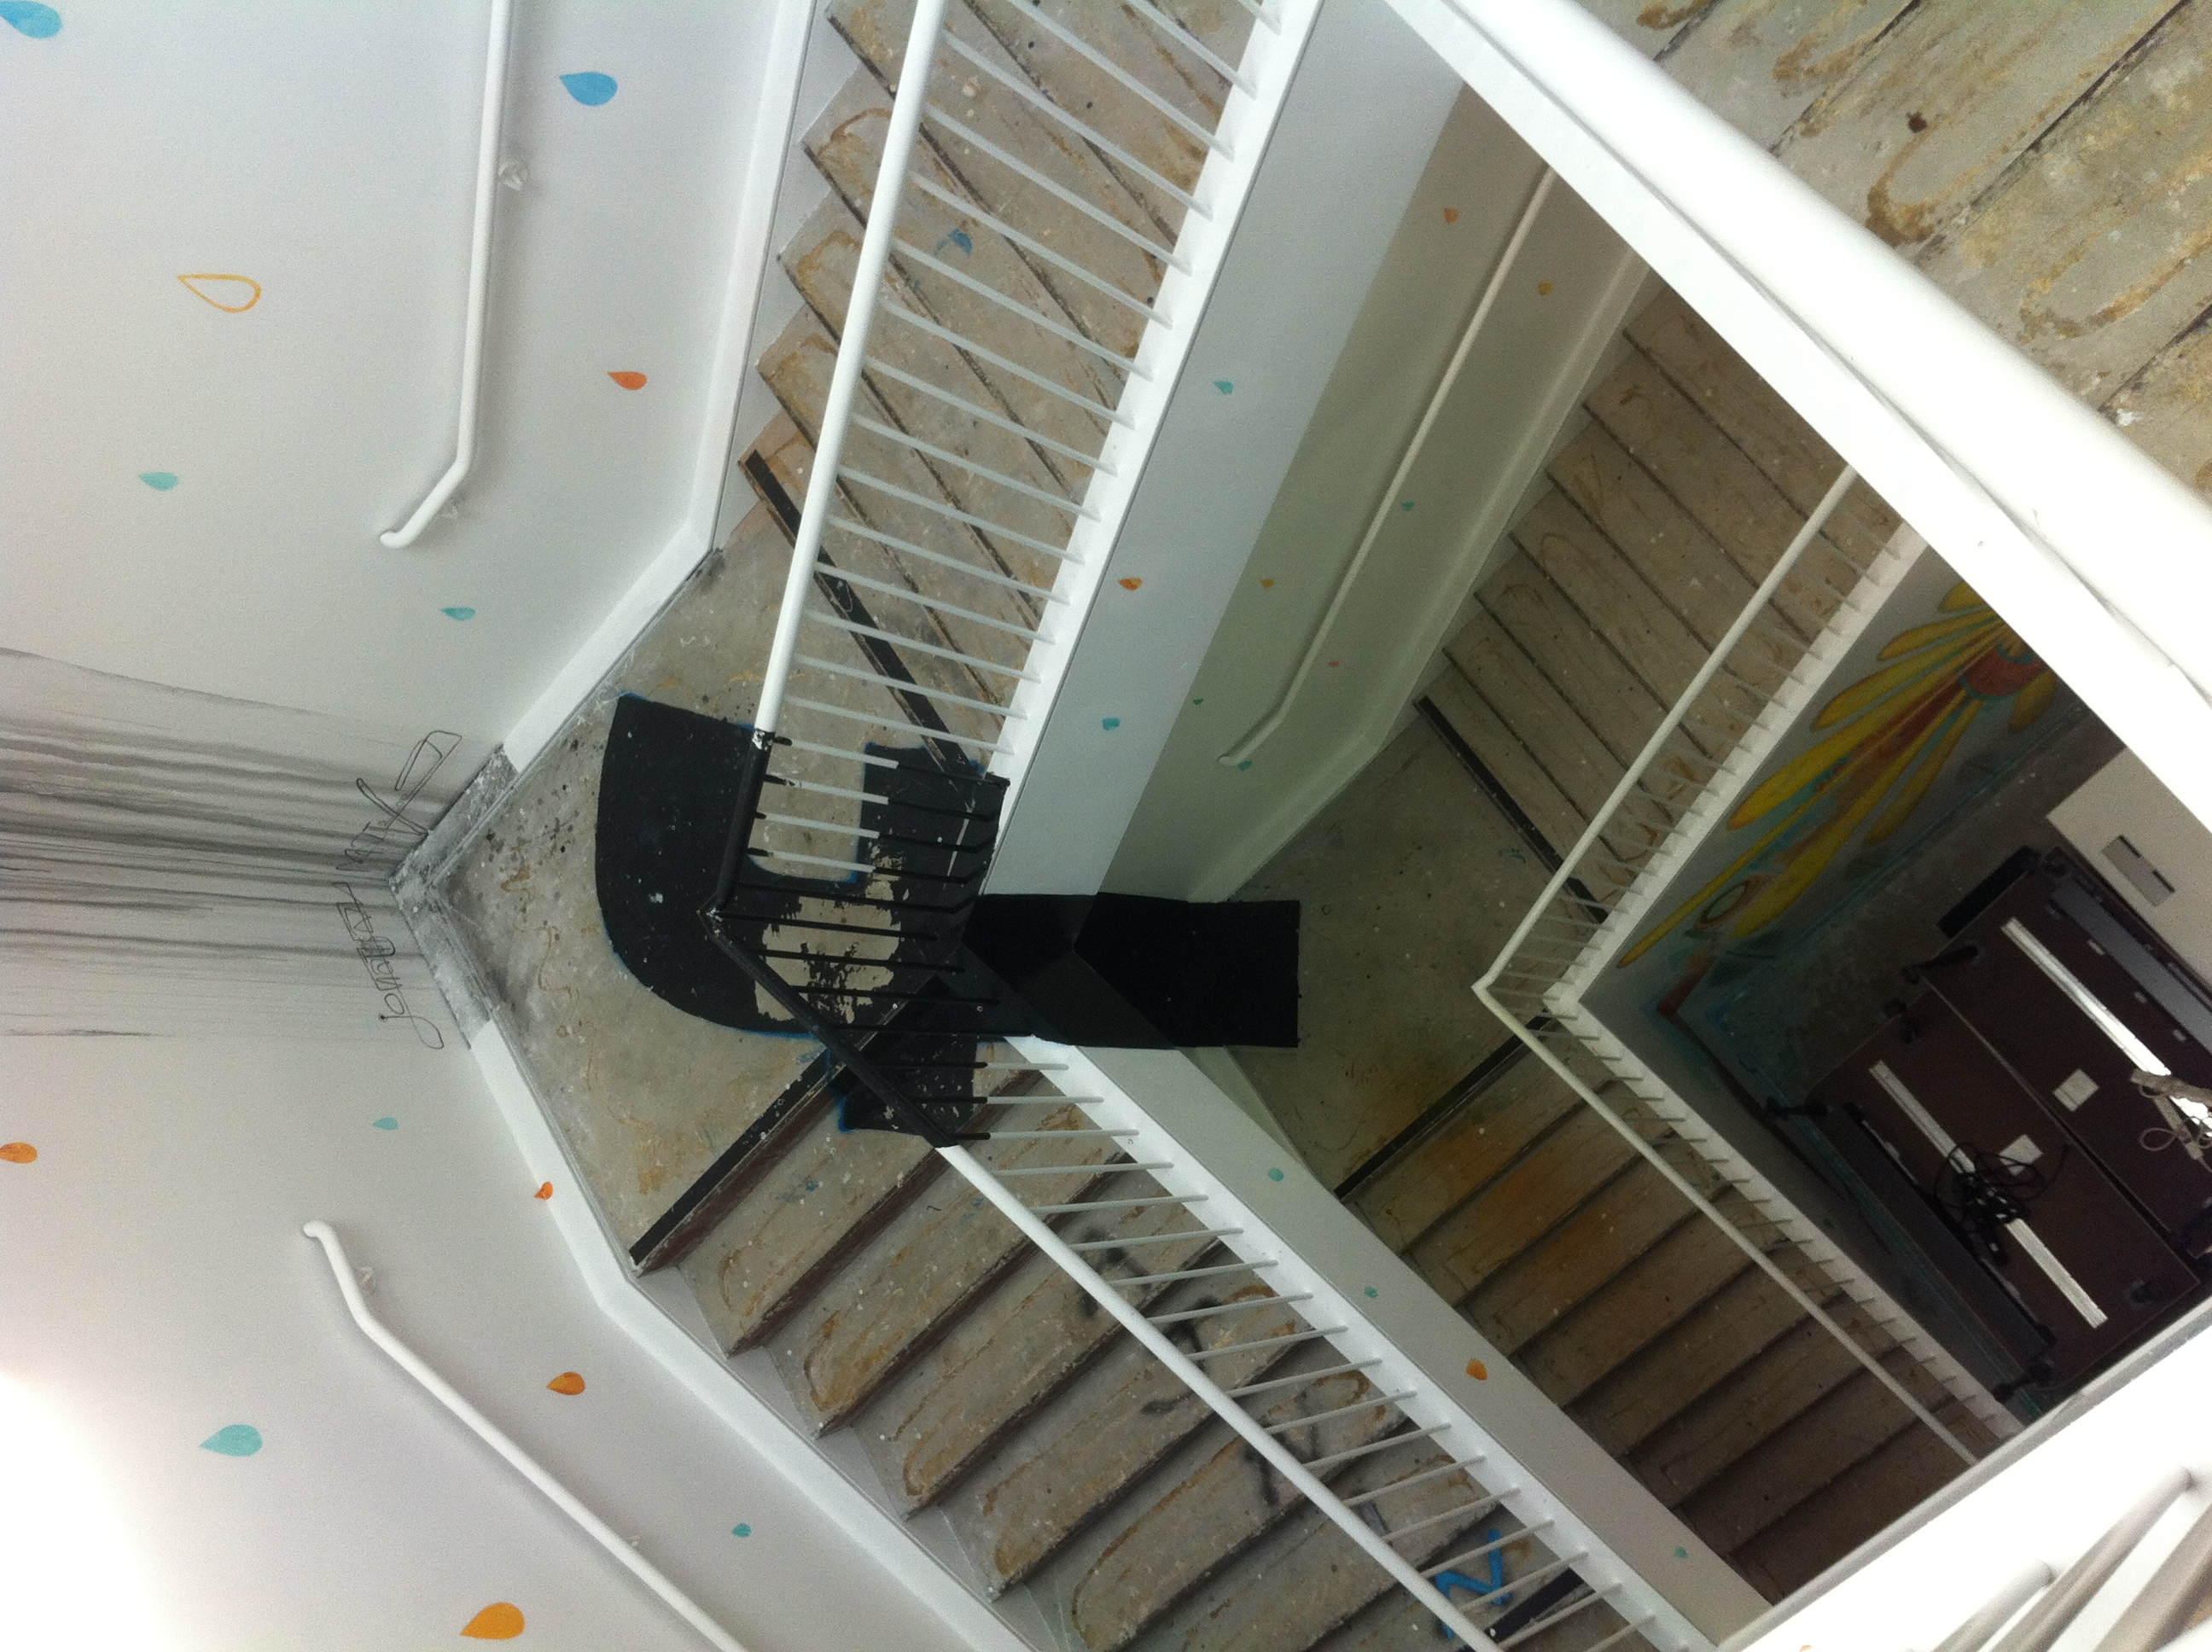
\includegraphics[width=.7\textwidth]{sntc/IMG_2067.JPG}
\end{center}
\end{block}
\end{frame}
\begin{frame}
\frametitle{Competições de Programação}
\begin{block}{Por que é Bom?}
\begin{center}
	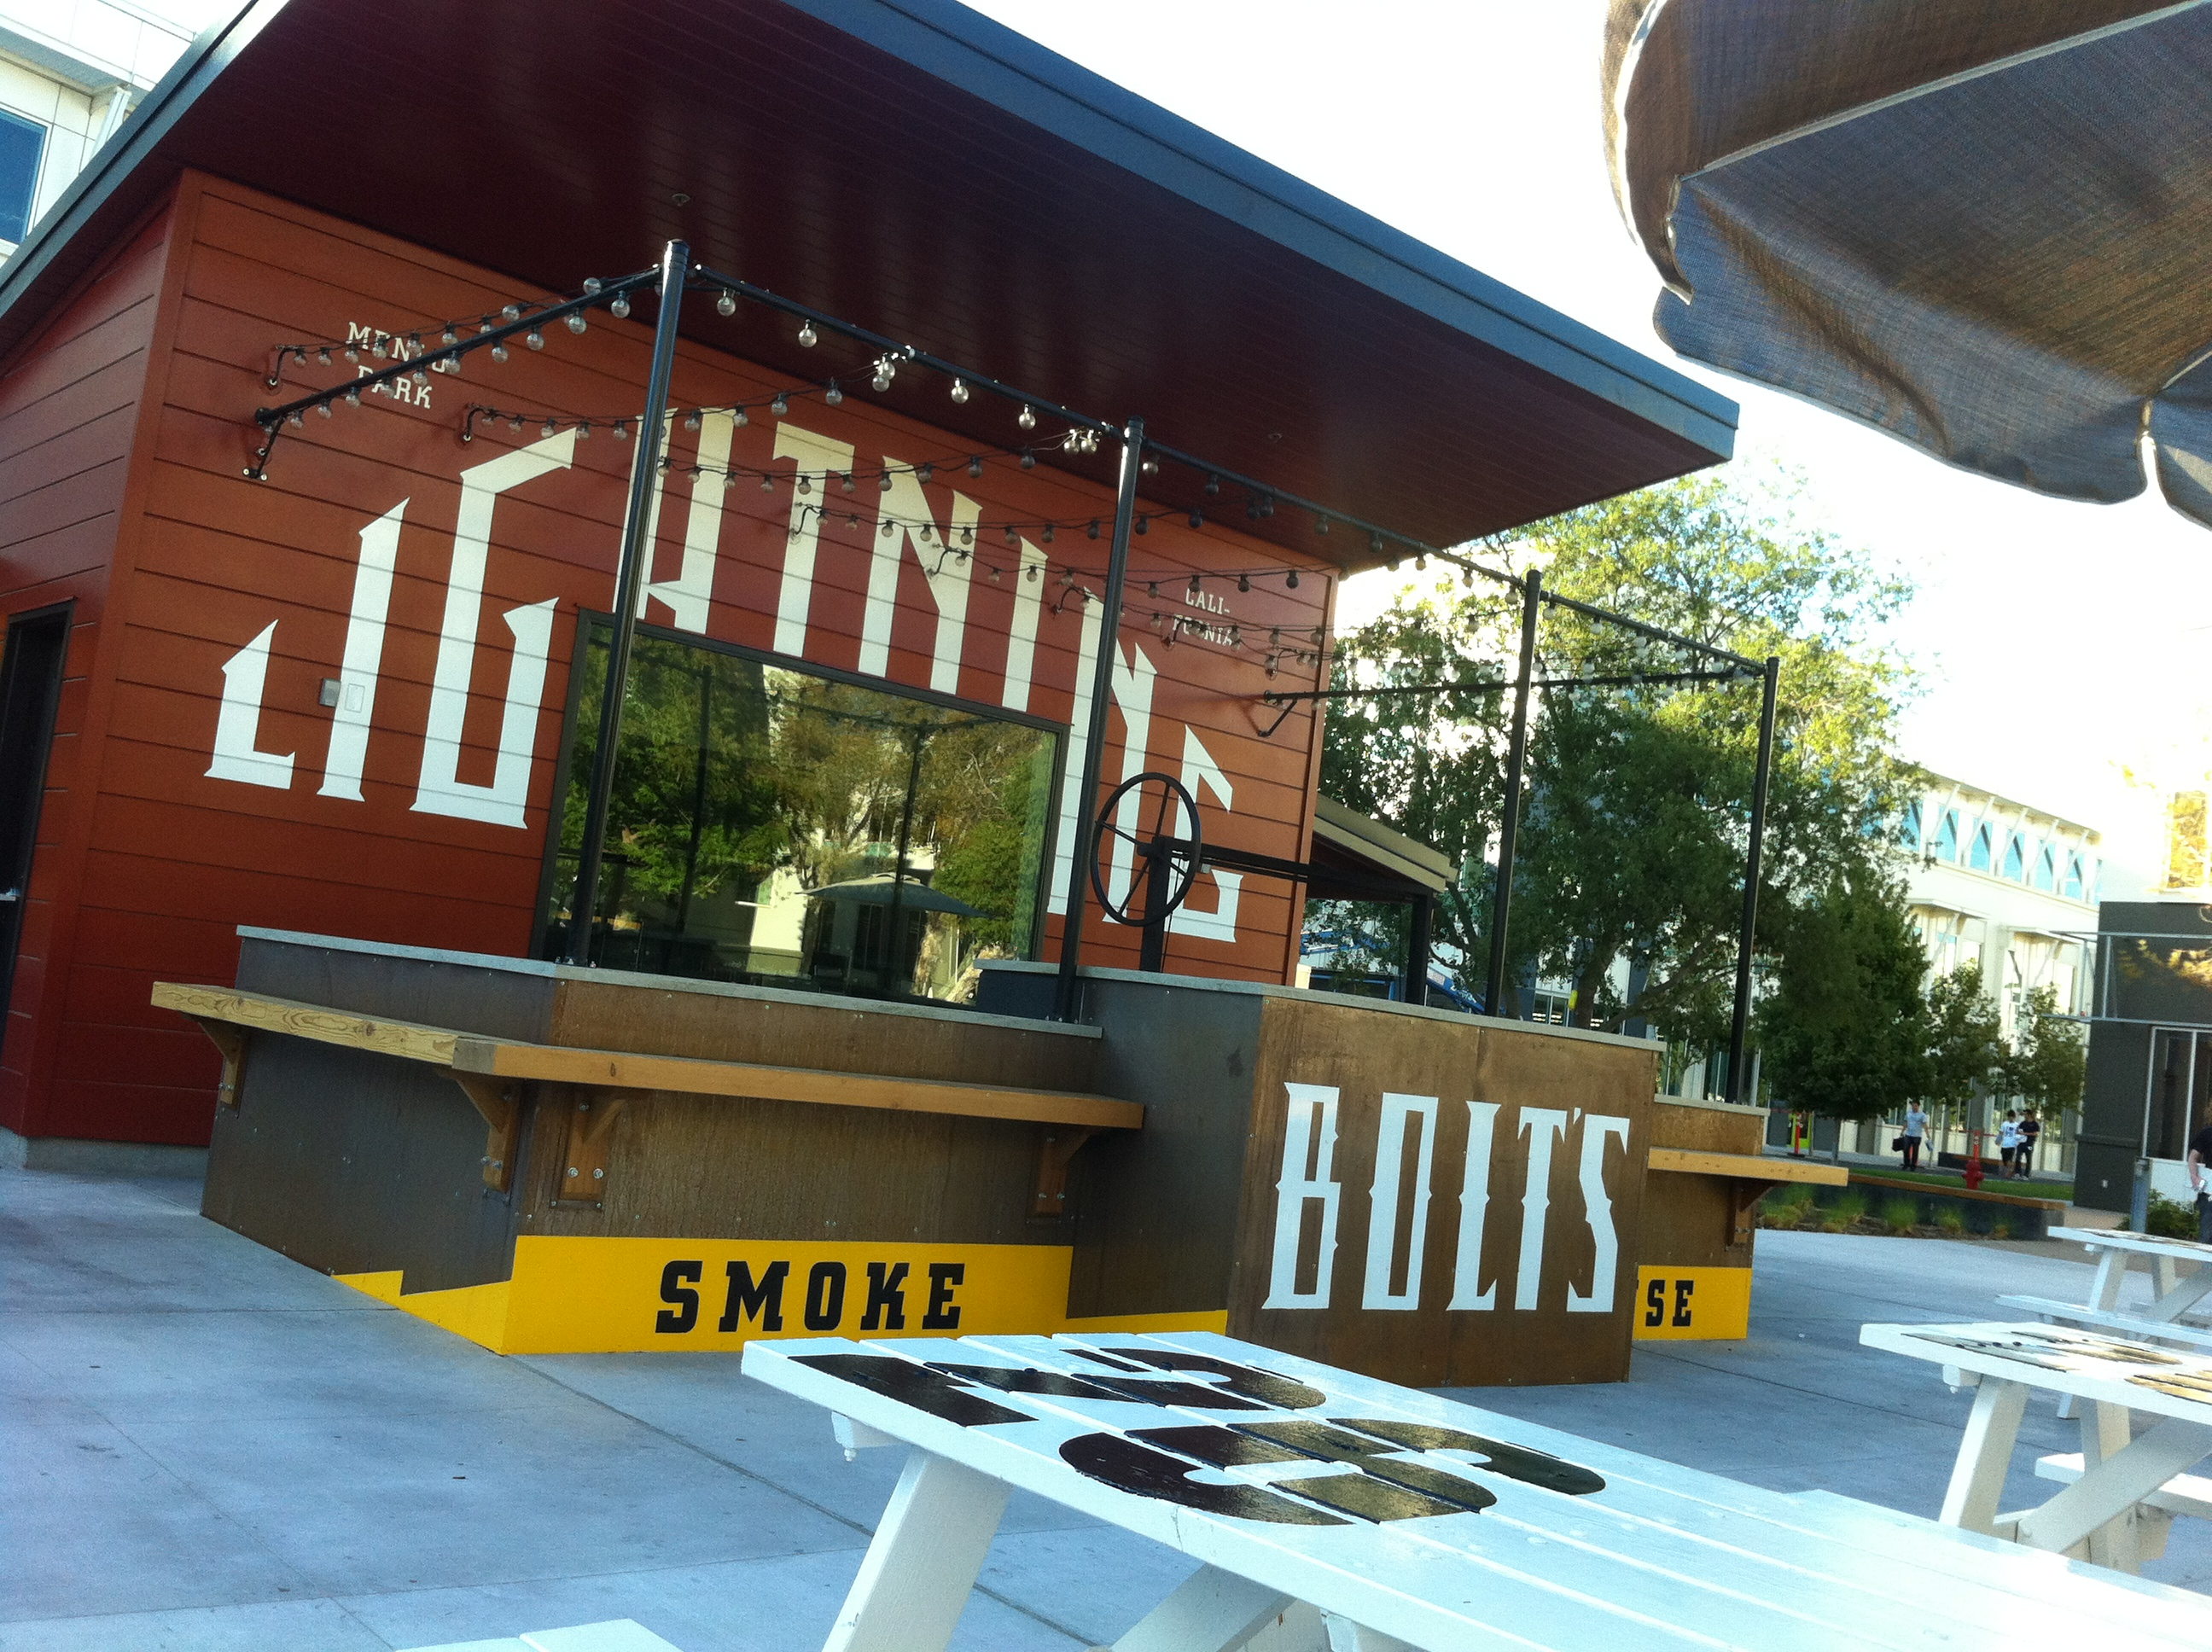
\includegraphics[width=.7\textwidth]{sntc/IMG_2074.JPG}
\end{center}
\end{block}
\end{frame}
\begin{frame}
\frametitle{Competições de Programação}
\begin{block}{Por que é Bom?}
\begin{center}
	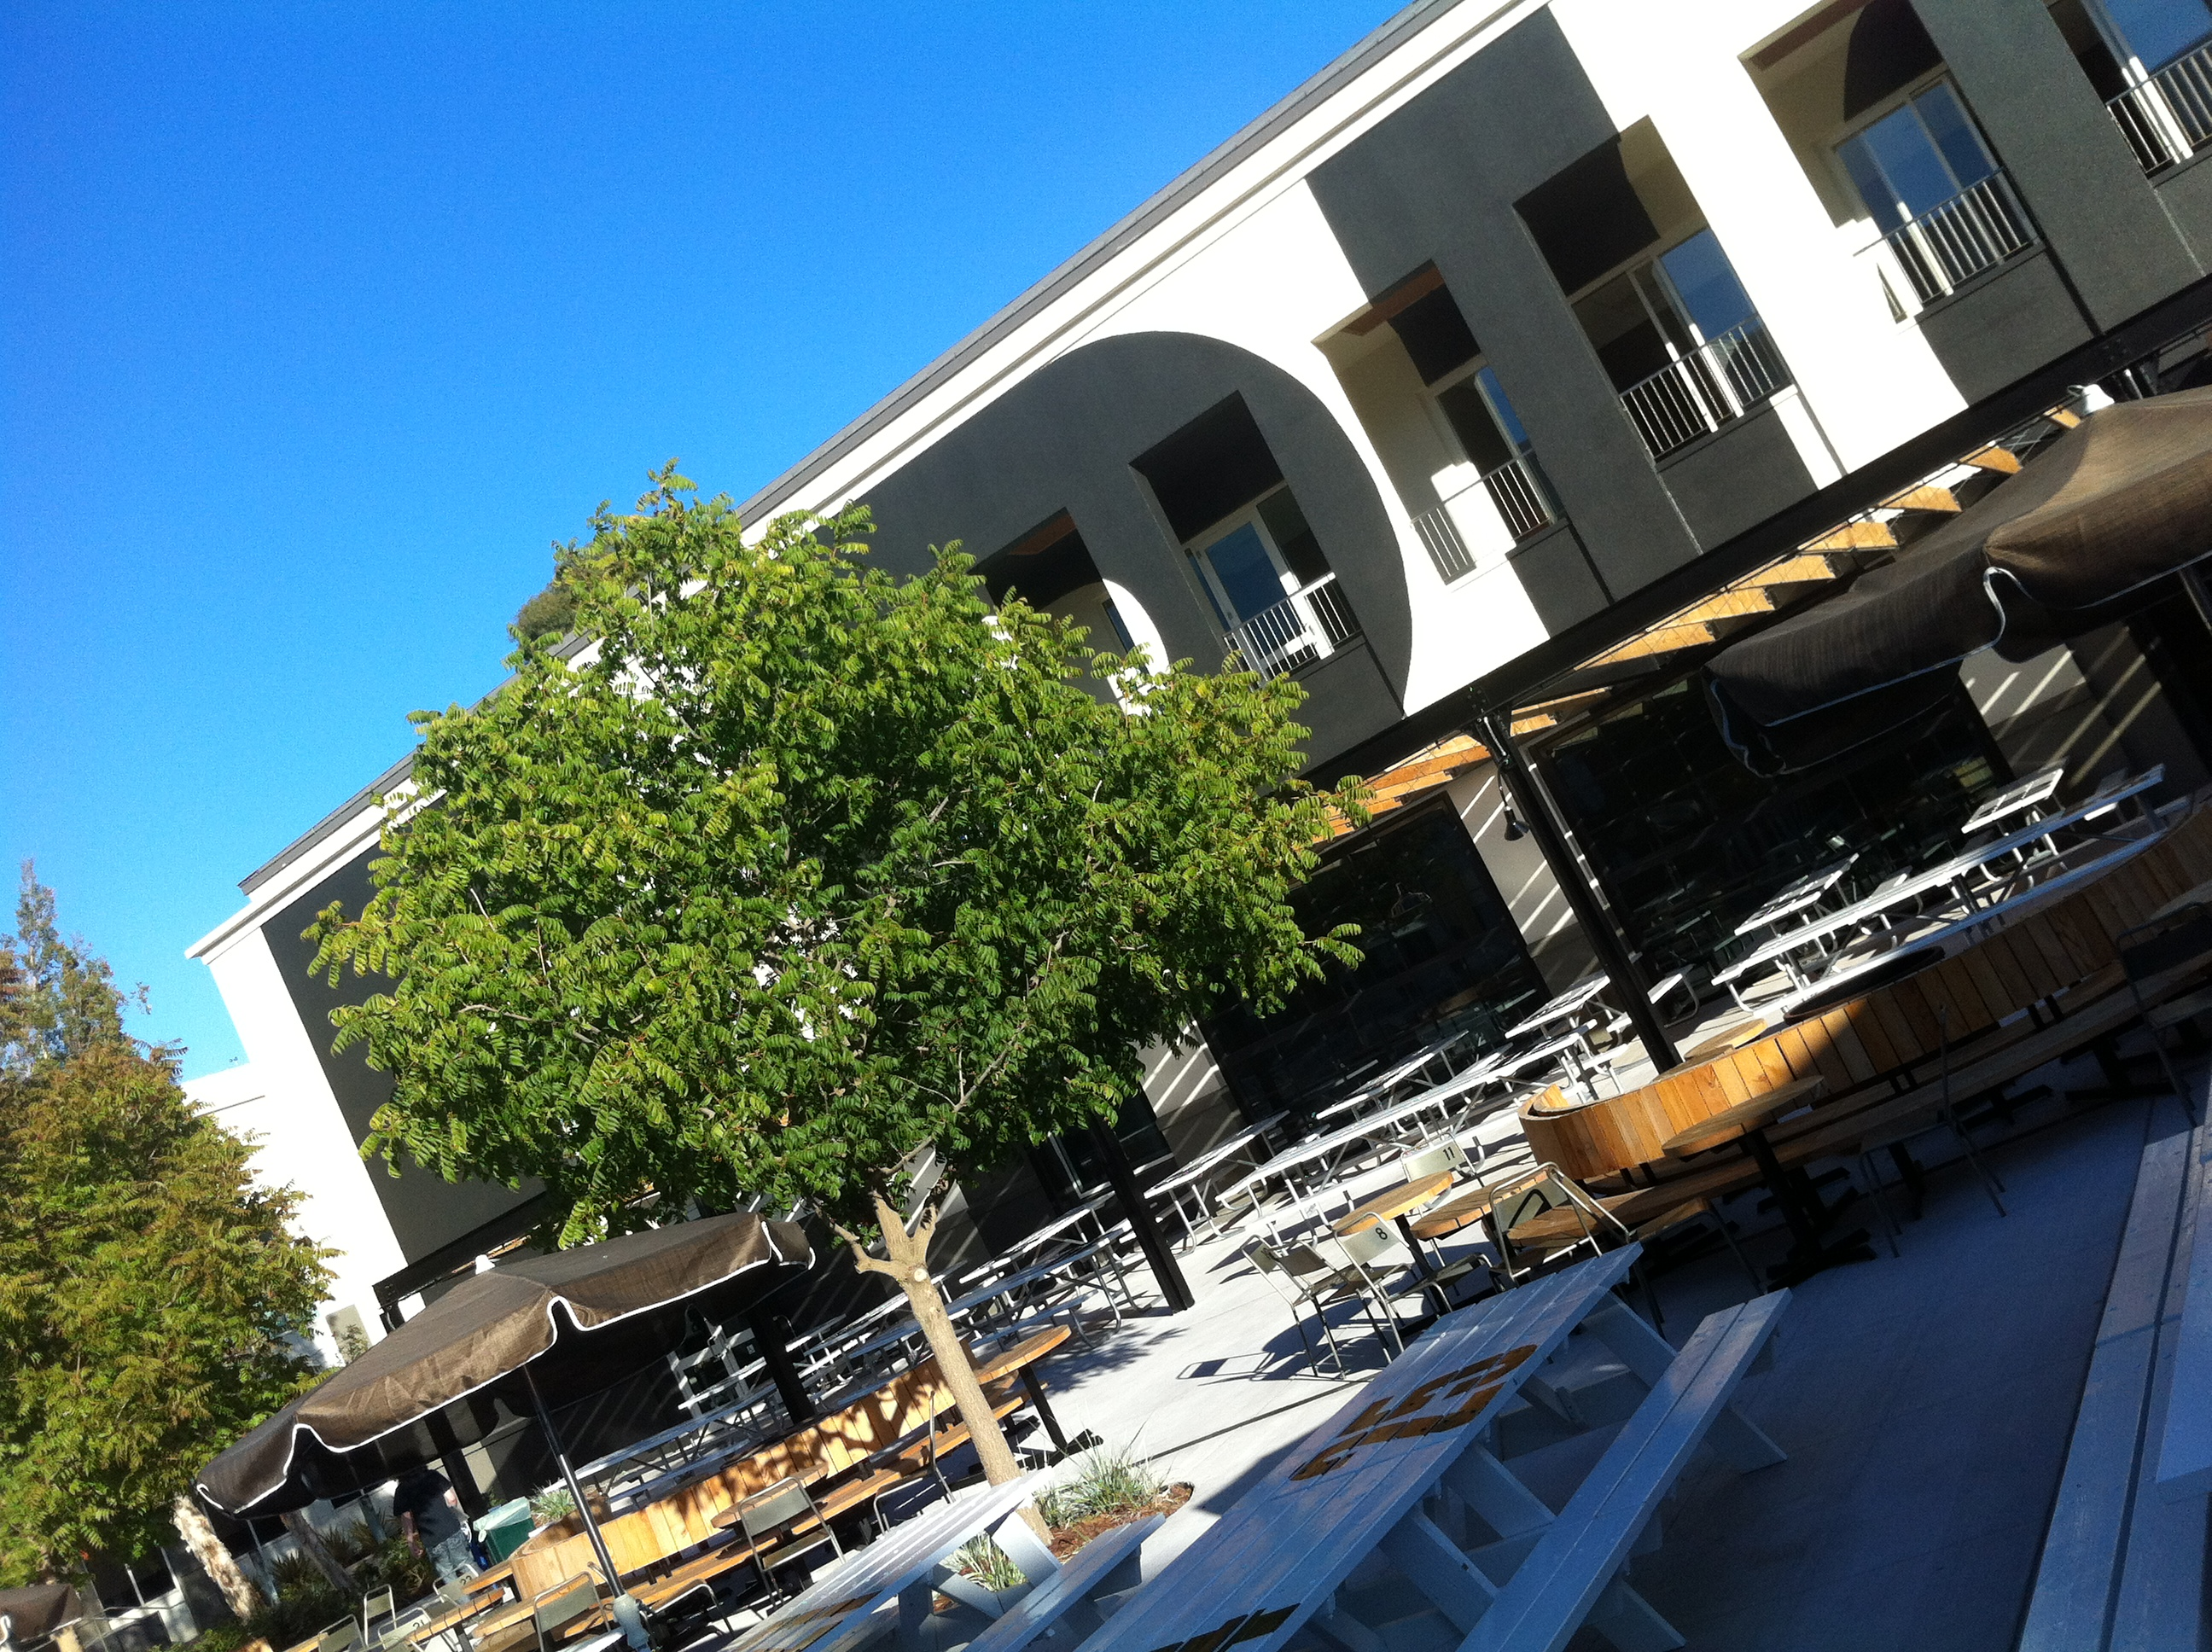
\includegraphics[width=.7\textwidth]{sntc/IMG_2075.JPG}
\end{center}
\end{block}
\end{frame}
%- - - - - - - - - - - - - - - - - - - - - - - - - - - - - - - - - SLIDES - SNCT
%- - - - - - - - - - - - - - - - - - - - - - - - - - - - - - - - -

%- - - - - - - - - - - - - - - - - - - - - - - - - - - - - - - - - SLIDE -
\begin{frame}
\frametitle{Competições de Programação}
\begin{block}{Como funcionam?}
\begin{itemize}
	\item Variam um pouco de estilo e regras, mas em todas é necessário programar.
	\item Existe um tempo fixo para resolver o conjunto de problemas propostos.
	\item Geralmente, para ganhar, você deve resolver o maior número de problemas no menor tempo possível.
\end{itemize}
\end{block}

\end{frame}
%- - - - - - - - - - - - - - - - - - - - - - - - - - - - - - - - - SLIDE -
\begin{frame}
\frametitle{Competições de Programação}
\begin{block}{Algumas competições}
\begin{itemize}
	\item Ensino médio: 
	\begin{itemize}
		\item Olimpíada Brasileira de Informática (OBI)
		\item International Olympiad in Informatics (IOI)
		\item TopCoder High School Tournament (TCHS)
	\end{itemize}
	\item Ensino superior: 
	\begin{itemize}
		\item Maratona de Programação
		\item ACM International Collegiate Programming Contest (ACM-ICPC)
		\item TopCoder Collegiate Challenge (TCCC)
	\end{itemize}
	\item Livre: 
	\begin{itemize}
		\item TopCoder Open (TCO)
		\item Google Code Jam (GCJ)
		\item Facebook Hacker Cup
		\item Internet Problem Solving Contest (IPSC)
		\item $\infty$
	\end{itemize}
\end{itemize}
\end{block}
\end{frame}
%- - - - - - - - - - - - - - - - - - - - - - - - - - - - - - - - - SLIDE -


\section{Maratona de Programação}
%- - - - - - - - - - - - - - - - - - - - - - - - - - - - - - - - - SLIDE -
\frame{
\frametitle{ICPC}
\begin{block}{}
\begin{itemize}
	\item {\em International Collegiate Programming Contest}
	\item Competição de programação existente desde 1970 e organizada pela ACM desde 1977.
	\item Patrocinada pela IBM.
	\item A missão do ICPC é dar oportunidades aos estudantes para interagir com alunos de outras universidades e demonstrar sua capacidade de {\bf resolver problemas}, {\bf programar} e {\bf trabalhar em grupo}.
\end{itemize}
\end{block}
}

%- - - - - - - - - - - - - - - - - - - - - - - - - - - - - - - - - SLIDE -
\frame{
\frametitle{ICPC}
\begin{block}{}
\begin{itemize}
	\item A competição possui duas etapas
	\begin{itemize}
		\item Finais Regionais -- realizadas localmente, em vários países ao redor do mundo. 
		\item Final Mundial -- reúne os melhores colocados das competições regionais.
	\end{itemize}
	
	\item A etapa regional ocorre no ano anterior à final mundial
	\begin{itemize}
		\item Os times se classificam nas regionais de 2012 para competir a final mundial de 2013.
	\end{itemize}
	
	\item Apenas um time por instituição é classificado para a final mundial.
\end{itemize}
\end{block}
}

%- - - - - - - - - - - - - - - - - - - - - - - - - - - - - - - - - SLIDE -
\begin{frame}
\frametitle{ICPC}
\begin{center}
	\begin{minipage}{.9\textwidth}
	\centering
	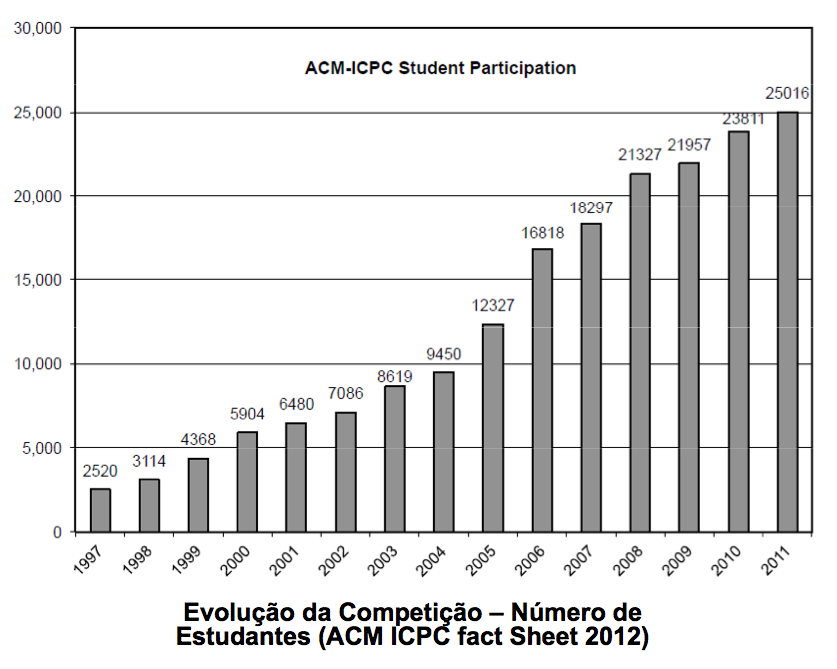
\includegraphics[width=.9\textwidth]{figuras/worldnmbrs.png}	
	\end{minipage}
\end{center}
\end{frame}

%- - - - - - - - - - - - - - - - - - - - - - - - - - - - - - - - - SLIDE -
\frame{
\frametitle{ICPC no mundo}
\begin{block}{}
\begin{itemize}
	\item 2007/2008: mais de 6700 times de 1821 escolas de 83 países.
	\begin{itemize}
		\item 100 participaram da Final Mundial do evento, em Banff, Canadá.
		\item Participação de 4 times brasileiros (IME, ITA, IME-USP, Unicamp) na final mundial.
	\end{itemize}

	\item 2011/2012: mais de 8338 times (mais de 25000 estudantes) de 2219 instituições de 88 países competiram em regionais nos 6 continentes.
	\begin{itemize}
		\item 112 times na Final Mundial do evento, em Varsóvia, Polônia.
		\item 6 times brasileiros (ITA,UFCG,UFPR,UFPE, UFRJ e IME-USP) participaram da final.
	\end{itemize}
\end{itemize}
\end{block}
}

%- - - - - - - - - - - - - - - - - - - - - - - - - - - - - - - - - SLIDE -
\begin{frame}
\frametitle{Maratona de Programação}
\begin{block}{ICPC no Brasil}
\begin{itemize}
	\item Maratona de Programação desde 1996.
	\item Realizada pela SBC desde o ano 2000.
	\item Apoio do CNPq desde 2002.
	\item Realizada em parceria com a Fundação Carlos Chagas desde o ano 2006.
\end{itemize}
\end{block}
\begin{center}
\begin{minipage}{.4\textwidth}
\frametitle{Maratona de Programação}
	\centering
	
\includegraphics[width=.75\textwidth]{logo/logomdp}
\end{minipage}
\end{center}
\end{frame}

%- - - - - - - - - - - - - - - - - - - - - - - - - - - - - - - - - SLIDE -
\begin{frame}
\frametitle{Maratona de Programação}
\begin{block}{Competição em duas fases}
\begin{description}[Sul Americana]
	\item [Regional] Classificatória para a final nacional.
	\item [Nacional] Final brasileira e classificatória para a final mundial.
\end{description}
\end{block}

\begin{block}{}
\small Na América do Sul existem três regionais do ICPC. 
\begin{itemize}
	\item \small South America/Brazil Regional -- A Final Nacional da Maratona de Programação.
	\item \small South America/North Regional -- Colômbia, Equador, Panamá, Venezuela.
	\item \small South America/South Regional -- Argentina, Bolívia, Chile, Peru, Paraguai, Uruguai.
\end{itemize}

\end{block}

\begin{block}{}
\begin{itemize}
	\item \url{http://maratona.ime.usp.br/}
	\item \url{http://www.inf.ufg.br/maratona/}
	\item \url{https://www.facebook.com/maratonago}
\end{itemize}
\end{block}
\end{frame}

%- - - - - - - - - - - - - - - - - - - - - - - - - - - - - - - - - SLIDE - 
\begin{frame}
\frametitle{Maratona de Programação}
\begin{center}
	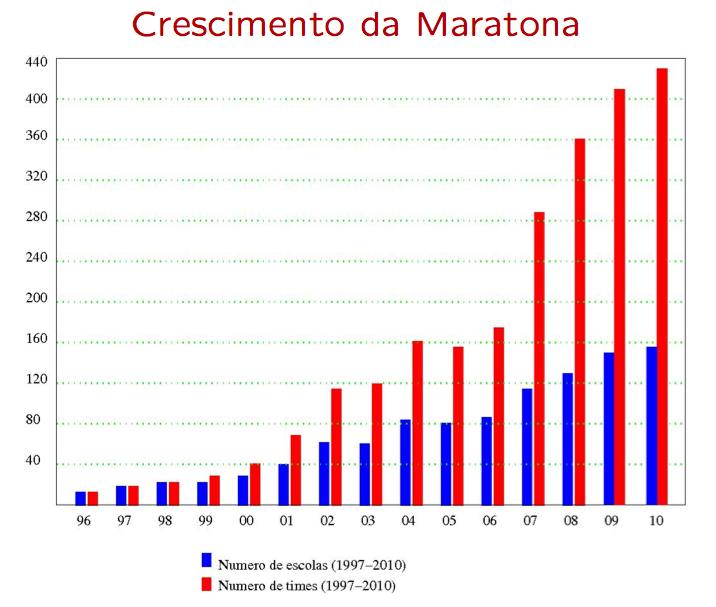
\includegraphics[width=.75\textwidth]{figuras/crescbrsl.png}
\end{center}
\end{frame}

%- - - - - - - - - - - - - - - - - - - - - - - - - - - - - - - - - SLIDE - 
\begin{frame}
\frametitle{Maratona de Programação}
\begin{center}
	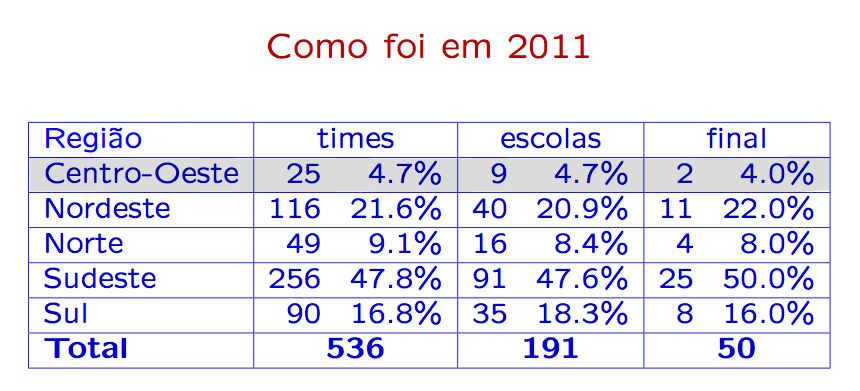
\includegraphics[width=.9\textwidth]{figuras/nmbrsl2.png}
\end{center}
\end{frame}

%- - - - - - - - - - - - - - - - - - - - - - - - - - - - - - - - - SLIDE -
\frame{
\frametitle{Maratona de Programação}
\begin{block}{Participação do INF - Fase Regional}
\centering
\begin{tabular}{ccccc}
\hline
{\bf Ano} & {\bf Local}       & {\bf Equipes} & {\bf Instituições} & {\bf Classificação} \\
\hline
2007     & Brasília-DF      & 5  & 3 & 3\textordmasculine \\
2008     & Goiânia-GO     & 7  & 3 & 1\textordmasculine\ e 3\textordmasculine \\
2009     & Goiânia-GO     & 11 & 4 &1\textordmasculine,3\textordmasculine\ e 4\textordmasculine \\
2010     & Goiânia-GO     & 10 & 3 &  1\textordmasculine, 4\textordmasculine, 6\textordmasculine\ e 8\textordmasculine \\
2011     & Goiânia-GO     & 14 & 4+1 & 1\textordmasculine, 2\textordmasculine, 5\textordmasculine\ e 8\textordmasculine \\
2012     & Goiânia-GO    & 10 & 3+1 & 1\textordmasculine, 2\textordmasculine, 3\textordmasculine\ , 6\textordmasculine\ e 8\textordmasculine \\
\hline
\end{tabular}
\end{block}
}

%- - - - - - - - - - - - - - - - - - - - - - - - - - - - - - - - - SLIDE -
\frame{
\frametitle{Maratona de Programação}
\begin{block}{Participação do INF - Final Brasileira}
\centering
\begin{tabular}{ccccc}
\hline
{\bf Ano} & {\bf Local}       & {\bf Equipes} & {\bf Instituições} & {\bf Classificação} \\
\hline
2008     & Vila Velha-ES & 51/360 & 129 & 28\textordmasculine\\
2009     & Campinas-SP & 52/410 & 145 & 22\textordmasculine\\ 
2010     & Joinville-SC & 51/432 & 157 & 20\textordmasculine\\
2011     & Goiânia-GO & 50/536 & 191 & 11\textordmasculine\\
2012     & Londrina-PR & 50/545 & 194 & 13\textordmasculine\\
\hline
\end{tabular}
\end{block}
}

%- - - - - - - - - - - - - - - - - - - - - - - - - - - - - - - - - SLIDE -
\begin{frame}
\frametitle{Maratona de Programação}
\begin{block}{Como funciona?}
\begin{itemize}
	\item Competição voltada para alunos de cursos de Ciência da Computação, Engenharia de Computação e áreas afins.
	\item Os times são compostos de três estudantes com até 5 anos de estudos universitários ou 23 anos de idade.
	\begin{itemize}
		\item Podem ter participado de no máximo 4 regionais e 1 final mundial.
	\end{itemize}
	\item Os times recebem de 8 a 12 problemas computacionais para serem resolvidos durante a competição (5 horas).
	\item Quando um time considera que resolveu um problema submete aos juízes que, {\em online}, dizem se a solução está ou não correta.
	\item Uma solução correta resolve um conjunto de testes dos juízes, desconhecido dos alunos e recebe um balão.
\end{itemize}
\end{block}
\end{frame}

%- - - - - - - - - - - - - - - - - - - - - - - - - - - - - - - - - SLIDE -
\begin{frame}
\frametitle{Maratona de Programação}
\begin{block}{Como funciona?}
\begin{itemize}
	\item Você deve saber programar em C, C++ ou Java.
	\item Cada equipe tem acesso a um computador, sem conexão à internet, e apenas a material impresso.
	\item Objetivo é apresentar soluções computacionalmente corretas para um dado problema no menor tempo possível.
	\begin{itemize}
		\item O time vencedor é aquele que resolver mais problemas durante as 5 horas de competição
		\item Em caso de empate vence o time com a menor ``penalidade''
		\begin{itemize}
			\item Soma das penalidades dos problemas corretamente resolvidos;
			\item A penalidade de um problema é dada pelo número de minutos decorridos desde o início da competição até o momento da primeira submissão correta;
			\item Uma penalidade de 20 minutos é adicionada por cada submissão incorreta feita antes da primeira submissão correta.
		\end{itemize}
   	\end{itemize}
\end{itemize}
\end{block}
\end{frame}

%- - - - - - - - - - - - - - - - - - - - - - - - - - - - - - - - - SLIDE -
\begin{frame}
\frametitle{Maratona de Programação}
\begin{block}{Como funciona?}
\begin{itemize}
	\item Cada problema contém:
	\begin{itemize}
		\item Informações para contextualização (Background)
		\item O enunciado do problema
		\item Informações sobre a entrada (Input)
		\item Informações sobre a saída (Output)
		\item Exemplo de entrada (Sample Input)
		\item Exemplo de saída (Sample Output)
	\end{itemize}
\end{itemize}
\end{block}
\end{frame}

%- - - - - - - - - - - - - - - - - - - - - - - - - - - - - - - - - SLIDE -
\begin{frame}
\frametitle{Maratona de Programação}
\begin{block}{Como funciona?}
\begin{itemize}
	\item Os juízes possuem datasets que são utilizados para testar a solução submetida
	\item Esses datasets contém instâncias de testes bastante diferentes dos exemplos contidos nos problemas do caderno de questões
	\item Os juízes informarão uma das seguintes respostas a uma solução submetida por um time (sem nenhum detalhe adicional)
	\begin{itemize}
		\item Yes
		\item No - Wrong Answer (WA)
		\item No - Presentation Error (PE)
		\item No - Time Limit Exceeded (TLE)
		\item No - Runtime Error (RE)
		\item No - Compile Error (CE)
	\end{itemize}
	\item O sistema não responde nada além disto. Não é possível saber, por exemplo, se um programa que recebeu TLE produz a saída correta, ou em qual linha está o erro de um programa que recebeu CE.

\end{itemize}
\end{block}
\end{frame}

%- - - - - - - - - - - - - - - - - - - - - - - - - - - - - - - - - SLIDE -
\begin{frame}
\frametitle{Maratona de Programação}
\begin{block}{E se eu me der bem?}
\begin{itemize}
	\item Os melhores colocados da primeira fase por sede avançam para a Final Nacional da Maratona de Programação.
	\item Medalhas aos 10 primeiros colocados na final nacional
	\begin{itemize}
		\item Ouro para os três primeiros
		\item Prata para os três seguintes
		\item Bronze para os quatro últimos
	\end{itemize}
	\item Cópia do Troféu ``Maratona de Programação'' para o vencedor
	\item Premiação para os melhores colocados de cada região
	\item Vencedor ganha vaga na Final Mundial do ICPC
	\begin{itemize}
		\item Outros \em{N} times melhores colocados podem ter direito a participar da Final Mundial, dependendo do nro. de vagas adicionais atribuídas ao Brasil.
	\end{itemize}
\end{itemize}
\end{block}
\end{frame}

%- - - - - - - - - - - - - - - - - - - - - - - - - - - - - - - - - SLIDE -
%\begin{frame}
%\frametitle{Maratona de Programação}
%\begin{block}{Objetivos}
%\begin{itemize}
%	\item Atrair o maior número de estudantes.
%	\item Atrair o maior número de escolas.
%	\item Envolver o maior número de países.
%	\item Prover condições iguais aos times para chegar às finais mundiais.
%	\item Criar competições disputadas.
%	\item Valorizar os estudantes e os voluntários.
%\end{itemize}
%\end{block}
%\end{frame}

\section{Como se preparar}
%- - - - - - - - - - - - - - - - - - - - - - - - - - - - - - - - - SLIDE -
\begin{frame}
\frametitle{Como Se Preparar?}
\begin{block}{}
Para estar bem preparado para participar dessas competições é necessário passar por varias etapas:
\begin{enumerate}
	\item Escolher uma linguagem;
	\begin{itemize}
		\item Dominar sintaxe, comandos básicos e as funções mais usadas em competições.
	\end{itemize}
	\item Aprender noções de Complexidade de Algoritmos;
	\begin{itemize}
		\item Calcular complexidade de tempo e memória e estimar o tempo de execução;
	\end{itemize}
	\item Dominar as estruturas de dados básicas;
	\begin{itemize}
		\item Vetores, strings, pilha, fila, etc.
	\end{itemize}
	\item Dominar Entrada e Saída;
	\begin{itemize}
		\item Leitura dos diferentes tipos, formatação de sáida.
	\end{itemize}
	\item Dominar algoritmos clássicos e técnicas comuns para resolução de problemas .
\end{enumerate}
\end{block}
\end{frame}

%- - - - - - - - - - - - - - - - - - - - - - - - - - - - - - - - - SLIDE -
\begin{frame}
\frametitle{Como Se Preparar?}
\begin{block}{Alguns exemplos de algoritmos clássicos e técnicas comuns}
\begin{itemize}	
	\item Recursão, Backtracking
	\begin{itemize}
		\item	Saber enumerar permutações, combinações e arranjos.
	\end{itemize}
	\item Grafos
	\begin{itemize}
		\item Estruturas de dados para representá-los; Algoritmos de busca: BFS, DFS; Árvore Geradora Mínima; Caminhos mínimos.
	\end{itemize}
	\item Programação Dinâmica
	\begin{itemize}	
		\item Entender a idéia e conhecer os problemas clássicos.
	\end{itemize}
	\item Matemática
	\begin{itemize}	
		\item Conceitos de combinatória, probabilidade, cálculo e teoria dos números.
	\end{itemize}
	\item Geometria / Geometria Computacional
	\item Algoritmos gulosos, divisão e conquista, estruturas de dados, ...
\end{itemize}
\end{block}
\end{frame}

%- - - - - - - - - - - - - - - - - - - - - - - - - - - - - - - - - SLIDE -
\begin{frame}
\frametitle{Como Se Preparar?}
\begin{block}{E como dominar essas técnicas?}
\begin{itemize}	
	\item Estudando as mesmas em livros, artigos e tutoriais encontrados na internet;
	\item Praticando em Online Judges;
	\begin{itemize}
		\item Existem várias páginas na internet onde é possível resolver problemas no estilo da maratona e conferir se sua solução está correta.
	\end{itemize}
	\item Participando de competições online;
	\begin{itemize}
		\item Vários Online Judges organizam competições para que os competidores possam treinar.
		\item Sites como topCoder, Codeforces e Codechef organizam competições regularmente.
	\end{itemize}
	\item Esclarecendo dúvidas e pedindo ajuda a competidores mais experientes.
\end{itemize}
\end{block}
\end{frame}

%- - - - - - - - - - - - - - - - - - - - - - - - - - - - - - - - - SLIDE -
\begin{frame}
\frametitle{Como Se Preparar?}
\begin{block}{Material para estudo - Livros voltados	 para competições}
\begin{itemize}
		\item Competitive Programming 2: This increases the lower bound of Programming Contests. Again. - Steven Halim, Felix Halim
		\item Programming Challenges - Steven S. Skiena, Miguel A. Revilla 
		\item The Art of Algorithms and Programming Contests. - Rujia Liu, Liang Huang 
		\item Art of Programming Contest - Ahmed Shamsul Arefin
\end{itemize}
\end{block}
\end{frame}

%- - - - - - - - - - - - - - - - - - - - - - - - - - - - - - - - - SLIDE -
\begin{frame}
\frametitle{Como Se Preparar?}
\begin{block}{Material para estudo - Referências para desenvolvimento de algoritmos}
\begin{itemize}
	\item Introduction to Algorithms. Thomas H. Cormen, Charles E. Leiserson, Ronald L. Rivest. MIT Press/MacGraw Hill, 1990. 
	\item Introduction to Algorithms: A Creative Approach. Udi Manber. Addison-Wesley, 1989. 
	\item Algorithms in C Parts 1-5. Robert Sedgewick. 3rd. Edition, vol. 1. Addison Wesley Longman, 1998. 
	\item Computational geometry: An introduction. F.P. Preparata and M.I. Shamos. Texts and Monographs in Computer Science, Springer-Verlag, New York, 1985. 
\end{itemize}
\end{block}
\end{frame}

%- - - - - - - - - - - - - - - - - - - - - - - - - - - - - - - - - SLIDE -
\begin{frame}
\frametitle{Como Se Preparar?}
\begin{block}{Material para estudo - Referências para desenvolvimento de algoritmos}
\begin{itemize}
	\item Grafos e Algoritmos Computacionais. J. L. Szwarcfiter. Campus, Rio de Janeiro, 1986. 
	\item Data Structures and Algorithms. Alfred V. Aho, Jhon E. Hopcroft and Jeffrey Ullman Addison Wesley, 1983. 
	\item Concrete Mathematics. Donald E. Knuth, Ronald L. Graham and O. Patashnik. 2nd Edition Addison-Wesley, 1994. 
	\item Computational Complexity. Papadimitriou, C.H., Addison-Wesley, 1993. 
\end{itemize}
\end{block}
\end{frame}

%- - - - - - - - - - - - - - - - - - - - - - - - - - - - - - - - - SLIDE -
\begin{frame}
\frametitle{Como Se Preparar?}
\begin{block}{Material para estudo - Uma ``bibliografia'' indicada}
\begin{itemize}
	\item Competitive Programming 2 - Steven Halim, Felix Halim
	\begin{center}
	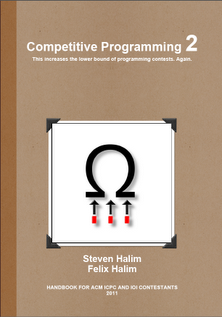
\includegraphics[width=.2\textwidth]{figuras/cp2.png}\\
	\tiny\url{https://sites.google.com/site/stevenhalim/}
	\end{center}
	
	\item \url{http://www.ime.usp.br/~pf/algoritmos_para_grafos/}
	\item \url{http://www.cplusplus.com/reference/}	
\end{itemize}
\end{block}
\end{frame}


%- - - - - - - - - - - - - - - - - - - - - - - - - - - - - - - - - SLIDE -
\begin{frame}
\frametitle{Como Se Preparar?}
\begin{block}{Online judges - A lista é extensa...}
\begin{itemize}
	\item URI Online Judge - \url{http://www.urionlinejudge.com.br/}
	\item UVa -- \url{http://uva.onlinejudge.org/}
	\item Live Archive -- \url{http://livearchive.onlinejudge.org/}
	\item SPOJ -- \url{http://www.spoj.pl/}
	\item TJU -- \url{http://acm.tju.edu.cn/toj/}
	\item SGU -- \url{http://acm.sgu.ru/}
	\item PKU -- \url{http://poj.org/}
	\item Timus -- \url{http://acm.timus.ru/}
	\item ZOJ -- \url{http://acm.zju.edu.cn/onlinejudge/}
	\item SPOJ BR  -- \url{http://br.spoj.pl/}
	\item USACO -- \url{http://train.usaco.org/usacogate}
	\item $\infty$
\end{itemize}
\end{block}
\end{frame}

%- - - - - - - - - - - - - - - - - - - - - - - - - - - - - - - - - SLIDE -
\begin{frame}
\frametitle{Como Se Preparar?}
\begin{block}{Online judges - Por once começar}
\begin{itemize}
	\item URI Online Judge - \url{http://www.urionlinejudge.com.br/}
	\begin{itemize}
		\item Portal brasileiro bastante didático com problemas em português e inglês classificados de acordo com a dificuldade e a possível técnica envolvida na solução.
	\end{itemize}
	\item SPOJ BR  -- \url{http://br.spoj.pl/}
		\begin{itemize}
		\item Página com problemas em português, de seletivas, regionais e nacionais passadas. Seção com problemas da OBI pode ser bastante interessante para alunos iniciantes.
	\end{itemize}
	\item USACO -- \url{http://train.usaco.org/usacogate}
	\begin{itemize}
		\item Curso de treinamento para os alunos dos Estados Unidos interessados em participar da olimpíada de informática. Dividido em seções, textos breves explicando técnicas e fornecendo mais referências e listas de problemas para serem resolvidos.
	\end{itemize}
\end{itemize}
\end{block}
\end{frame}

%- - - - - - - - - - - - - - - - - - - - - - - - - - - - - - - - - SLIDE -
\begin{frame}
\frametitle{Como Se Preparar?}
\begin{block}{Online judges - Partindo para problemas mais desafiadores}
\begin{itemize}
	\item SPOJ -- \url{http://www.spoj.pl/}	
	\begin{itemize}
		\item Coleção vasta de problemas com enunciados em inglês de origens e dificuldades variadas.
	\end{itemize}
	\item Live Archive -- \url{http://livearchive.onlinejudge.org/}
	\begin{itemize}
		\item Coleção de problemas das provas de regionais e finais mundiais passadas.
	\end{itemize}
	\item UVa -- \url{http://uva.onlinejudge.org/}
\end{itemize}
\end{block}
\end{frame}

%- - - - - - - - - - - - - - - - - - - - - - - - - - - - - - - - - SLIDE -
\begin{frame}
\frametitle{Como Se Preparar?}
\begin{block}{Online judges - Ferramentas}
\begin{itemize}
	\item Virtual Online Contests -- \url{http://ahmed-aly.com/voc/}
	\begin{itemize}
		\item Permite criar placares para competições envolvendo problemas de vários juízes e acompanhar quais problemas os usuários resolveram. Também tem vários outros recursos, como buscar por problemas de acordo com a técnica envolvida na solução e criar times e grupos.
	\end{itemize}
	\item uHunt -- \url{http://uhunt.felix-halim.net/}	
	\begin{itemize}
		\item Ferramenta para o UVa online-judge que gera estatísticas dos problemas resolvidos por cada usuário e dá sugestões de quais problemas resolver. Criado por um dos autores do livro Competitive Programming facilita bastante encontrar e manter um histórico de quais dos problemas discutidos no livro já foram resolvidos.
	\end{itemize}
\end{itemize}
\end{block}
\end{frame}

%- - - - - - - - - - - - - - - - - - - - - - - - - - - - - - - - - SLIDE -
\begin{frame}
\frametitle{Como Se Preparar?}
\begin{block}{Competições Online}
\begin{itemize}
	\item TopCoder SRMs -- \url{http://topcoder.com/tc}
	\item Codeforces -- \url{http://codeforces.com/contests}
	\item Codechef -- \url{http://codechef.com/}
	\item TopCoder Open -- \url{http://community.topcoder.com/tco13/}	
	\item Google Code Jam -- \url{http://code.google.com/codejam/}
	\item Facebook Hacker Cup -- \url{https://www.facebook.com/hackercup}
	\item IPSC -- \url{http://ipsc.ksp.sk/}
	\item \bf{Calendário de competições} -- \url{http://codingdoor.com/}
\end{itemize}
\end{block}
\end{frame}

%- - - - - - - - - - - - - - - - - - - - - - - - - - - - - - - - - SLIDE -
\begin{frame}
\frametitle{Como Se Preparar?}
\begin{block}{Competições Online -- TopCoder}
\begin{itemize}
	\item TopCoder SRMs -- \url{http://topcoder.com/tc}
	\begin{itemize}
		\item Geralmente ocorrem de 15 em 15 dias. 
		\item Competidores recebem uma pontuação e são rankeados e separados em divisões. Div. 2 tem problemas mais simples, a medida que o competidor vai apresentando um bom desempenho sua pontuação aumenta e ele passa a competir na div. 1 onde os problemas são mais desafiadores.
		\item Competição dividida em fases: Coding Phase, Challenge Phase e System Test.
		\item Explicações das soluções para os problemas divulgadas algum tempo após a competição.
	\end{itemize}
\end{itemize}
\end{block}
\end{frame}

%- - - - - - - - - - - - - - - - - - - - - - - - - - - - - - - - - SLIDE -
\begin{frame}
\frametitle{Como Se Preparar?}
\begin{block}{Competições Online -- TopCoder}
\begin{center}
	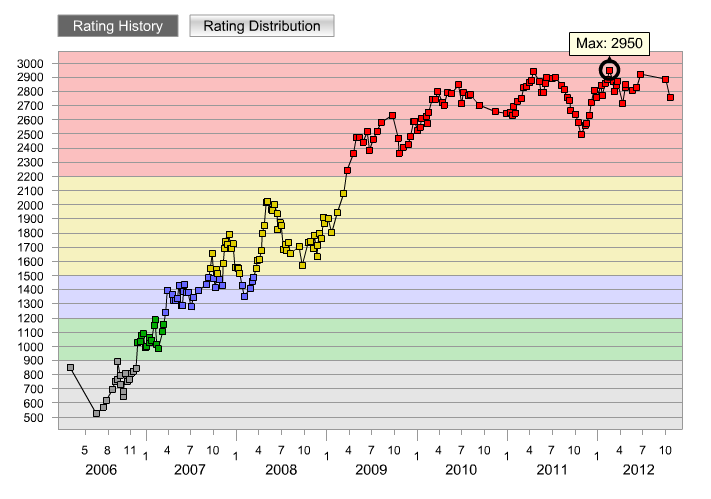
\includegraphics[width=.7\textwidth]{figuras/tcrating.png}
\end{center}
\end{block}
\end{frame}
	
%- - - - - - - - - - - - - - - - - - - - - - - - - - - - - - - - - SLIDE -	
\begin{frame}
\frametitle{Como Se Preparar?}
\begin{block}{Competições Online -- Codeforces}
\begin{itemize}	
	\item Codeforces -- \url{http://codeforces.com/contests}
	\begin{itemize}
		\item Competições semelhantes as do topCoder, porém com mais problemas e maior duração. Os competidores são separados em duas divisões e as competições tem duas etapas, Coding Phase e System Test.
		\item Explicações das soluções para os problemas geralmente são divulgadas algum tempo após a competição.
	\end{itemize}
\end{itemize}
\end{block}
\end{frame}

%- - - - - - - - - - - - - - - - - - - - - - - - - - - - - - - - - SLIDE -
\begin{frame}
\frametitle{Como Se Preparar?}
\begin{block}{Competições Online -- Codechef}
\begin{itemize}	
	\item Codechef -- \url{http://codechef.com/}
	\begin{itemize}
		\item Dois tipos de competições, ambas sem distinção entre os competidores.
		\begin{itemize}
			\item Long Contests -- Competição mais didática e de longa duração, acontece todos os meses a partir do dia primeiro e tem duração de 10 dias. A prova é composta por 10 problemas de dificuldades variadas e o objetivo é que o competidor tenha tempo de pesquisar e aprender novas técnicas para resolver os problemas propostos. 
			\item Short Contests -- Competições curtas, com 2,5 horas de duração que acontecem uma vez por mês. A prova tem 5 questões de dificuldades variadas.
		\end{itemize}
		\item Explicações das soluções sempre são divulgadas pouco tempo depois das competições.
	\end{itemize}
\end{itemize}
\end{block}
\end{frame}

%- - - - - - - - - - - - - - - - - - - - - - - - - - - - - - - - - SLIDE -
\begin{frame}
\frametitle{Como Se Preparar?}
\begin{block}{Entrar em contato com outros competidores}
\begin{itemize}	
	\item Praticamente todos os Online Judges tem fóruns onde os usuários podem trocar informações e dicas sobre os problemas, é importante usar bastante essa ferramenta.
	\item \url{http://br.groups.yahoo.com/group/maratona/} -- Grupo nacional da maratona no Yahoo Grupos, lugar onde competidores de todo o Brasil podem discutir sobre resoluções de problemas e competições de programação.
	\item \url{https://www.facebook.com/groups/maratonago/} -- Grupo destinado a alunos, professores, ex-competidores e entusiastas da Maratona de Programação no estado de Goiás. 
\end{itemize}
\end{block}
\end{frame}

%- - - - - - - - - - - - - - - - - - - - - - - - - - - - - - - - - SLIDE -
%\begin{frame}
%\frametitle{Como Se Preparar?}
%\begin{block}{Mais alguns endereços \dots}
%\begin{itemize}
%	\item \url{https://sites.google.com/site/obiufg/Principal} -- Página do treinamento da OBI oferecido pelo INF-UFG, livro preparatório para OBI pode ser encontrado nesse link.
%	\item \url{http://www.ime.usp.br/~cassio/boca/} -- site do BOCA
%\end{itemize}
%\end{block}
%\end{frame}

%- - - - - - - - - - - - - - - - - - - - - - - - - - - - - - - - - SLIDE -
%\begin{frame}
% \frametitle{\em Universidade de Valladolid}
% \begin{block}{}%{Online Judge}
%  \centering
%  \includegraphics[width=.95\textwidth]{figuras/uva-online-judge}
% \end{block}
%\end{frame}

\section{Dúvidas?}

\end{document}

